\documentclass[11pt,a4paper]{article}

\usepackage[utf8]{inputenc}
\usepackage[T1]{fontenc}
\usepackage[catalan]{babel}
\usepackage{lmodern}
\usepackage[a4paper,margin=2.0cm]{geometry}
\usepackage{amsmath}
\usepackage{graphicx}
\usepackage{booktabs}
\usepackage[dvipsnames,table]{xcolor}
\usepackage{listings}
\usepackage{needspace}
\usepackage{placeins}
\usepackage{caption}
\usepackage{tikz}
\usetikzlibrary{positioning,arrows.meta,shapes.multipart}
\usepackage[colorlinks=true,linkcolor=MidnightBlue,urlcolor=MidnightBlue,citecolor=MidnightBlue]{hyperref}

\setlength{\parskip}{4pt}
\setlength{\emergencystretch}{3em}
\renewcommand{\topfraction}{0.9}
\renewcommand{\bottomfraction}{0.8}
\renewcommand{\textfraction}{0.07}
\renewcommand{\floatpagefraction}{0.8}
\captionsetup{font=small,labelfont=bf}

\definecolor{codifons}{rgb}{0.97,0.97,0.97}
\definecolor{codiclau}{rgb}{0.0,0.0,0.85}
\definecolor{codicoment}{rgb}{0.13,0.55,0.13}
\definecolor{codicadena}{rgb}{0.63,0.13,0.94}
\lstset{language=Matlab, basicstyle=\ttfamily\footnotesize, keywordstyle=\color{codiclau}, commentstyle=\color{codicoment}, stringstyle=\color{codicadena}, backgroundcolor=\color{codifons}, frame=single, rulecolor=\color{gray!60}, framerule=0.4pt, columns=fullflexible, keepspaces=true, breaklines=true, showstringspaces=false, upquote=true, aboveskip=8pt, belowskip=6pt, captionpos=t}
\renewcommand{\lstlistingname}{Codi}

\title{\textbf{Un dron autònom que busca l'origen d'una fuga}\\[4pt]\large Arquitectura del codi, model de la ploma i algorismes de cerca}
\author{Projecte \texttt{Dron\_simon}}
\date{\today}

\begin{document}

\maketitle

\begin{abstract}
Presentem \texttt{Dron\_simon}, un simulador en MATLAB d'un dron autònom que ha de localitzar l'origen d'una fuga de contaminant fent servir només les lectures d'un sensor químic. Descrivim l'arquitectura del codi, organitzada en tres mòduls amb programació orientada a objectes; la generació de quatre versions de ploma (gaussiana o turbulenta, en 2D o 3D), que es guarden com a matrius espaciotemporals en fitxers NetCDF; el model del dron i del seu sensor; i els dos algorismes de cerca que hem implementat: l'\emph{infotaxis}, basat en inferència bayesiana i teoria de la informació, i un algorisme de \emph{gradient} amb cerca en zig-zag. Acabem amb els resultats de les vuit combinacions i amb el treball futur.
\end{abstract}

\setcounter{tocdepth}{1}
\tableofcontents

\section{Introducció}

L'objectiu del projecte és simular un dron que localitza l'origen d'una fuga de contaminant (per exemple, un gas tòxic en una zona industrial) sense saber on és. El dron només disposa de les lectures d'un sensor químic i de la direcció mitjana del vent. A cada pas mesura, actualitza el que sap i decideix cap on es mou, fins que arriba a tocar de la fuga o s'esgota l'autonomia.

El problema és difícil per dos motius. Primer, la ploma de contaminant no és un núvol suau: el vent és turbulent, amb remolins i canvis de direcció aleatoris, i el gas arriba al sensor de manera intermitent, a ràfegues. El dron pot passar molts segons sense detectar res encara que sigui a prop de la fuga, i per tant no pot limitar-se a pujar per la concentració. Segon, el sensor és sorollós: dues mesures al mateix lloc i al mateix instant no donen el mateix valor.

El simulador permet combinar tres opcions, que donen $2 \times 2 \times 2 = 8$ casos:
\begin{itemize}
\item \textbf{Dimensió}: \texttt{'2d'} (el dron vola a l'alçada de la fuga i només busca en horitzontal) o \texttt{'3d'} (no coneix l'alçada de la fuga i també es mou en vertical).
\item \textbf{Ploma}: \texttt{'gaussiana'} (estacionària, és a dir, constant en el temps) o \texttt{'complexa'} (turbulenta i variable en el temps).
\item \textbf{Algorisme}: \texttt{'infotaxis'} (manté un mapa de probabilitat de la posició de la fuga i maximitza la informació que espera obtenir) o \texttt{'gradient'} (segueix la direcció en què creix la concentració).
\end{itemize}

\section{Arquitectura del programari}

\subsection{Tres mòduls amb responsabilitats separades}

Hem dividit el codi en tres fitxers (taula~\ref{tab:fitxers}) seguint el principi de \emph{separació de responsabilitats}: cada mòdul s'encarrega d'una sola cosa i es comunica amb els altres a través d'una interfície petita i ben definida. La decisió de disseny més important és que la ploma i el dron no es coneixen entre ells: la ploma es genera i es desa en un fitxer, i el dron només llegeix les dades d'aquest fitxer. D'aquesta manera podem substituir la ploma per una altra (per exemple, una simulació atmosfèrica realista) sense tocar ni una línia del dron.

\begin{table}[htbp]
\centering
\caption{Els tres mòduls del projecte.}
\label{tab:fitxers}
\begin{tabular}{@{}lp{11.8cm}@{}}
\toprule
Fitxer & Responsabilitat \\
\midrule
\texttt{main.m} & Punt d'entrada: opcions, escenari, bucle de simulació (\texttt{simular}) i visualització. \\
\texttt{Ploma.m} & Genera les quatre versions de ploma com una matriu de concentracions amb dimensió temporal i la desa i llegeix en format NetCDF. \\
\texttt{Dron.m} & Classe \texttt{Dron}: paràmetres, graella de moviment, sensor i els algorismes infotaxis i gradient. No depèn de \texttt{Ploma.m}. \\
\bottomrule
\end{tabular}
\end{table}

\subsection{Flux de dades}

La figura~\ref{fig:flux} resumeix el flux de dades. \texttt{Ploma.generar} calcula la matriu de concentracions, \texttt{Ploma.guardar} l'escriu en un fitxer \texttt{.nc} i \texttt{Ploma.llegir} la carrega en una estructura \texttt{camp}. Una \emph{struct} de MATLAB és un contenidor amb camps amb nom (\texttt{camp.x}, \texttt{camp.c}\ldots); en el nostre cas, \texttt{camp} té els eixos \texttt{x}, \texttt{y}, \texttt{z}, \texttt{t}, la matriu \texttt{c} i la posició de la fuga \texttt{posFuga}. Aquesta \emph{struct} és tota la interfície entre la ploma i el dron. Finalment, la funció \texttt{simular} fa volar el dron dins del camp.

\begin{figure}[htbp]
\centering
\begin{tikzpicture}[node distance=5mm and 16mm, caixa/.style={draw=MidnightBlue, fill=MidnightBlue!8, rounded corners=2pt, rectangle, align=center, inner sep=5pt, font=\small, minimum height=12mm}, fletxa/.style={-{Stealth[length=2.5mm]}, thick, MidnightBlue}]
\node[caixa] (gen) {\texttt{Ploma.generar}\\matriu $c(x,y,z,t)$};
\node[caixa, right=of gen] (nc) {fitxer\\\texttt{ploma\_\ldots.nc}};
\node[caixa, right=of nc] (lle) {\texttt{Ploma.llegir}\\struct \texttt{camp}};
\node[caixa, below=8mm of lle] (sim) {\texttt{simular}: a cada pas\\\texttt{dron.pas(camp)}\\\texttt{dron.veuFuga(...)}};
\node[caixa, left=of sim] (res) {resultat \texttt{res}\\i figures};
\draw[fletxa] (gen) -- node[above, font=\footnotesize]{\texttt{guardar}} (nc);
\draw[fletxa] (nc) -- (lle);
\draw[fletxa] (lle) -- (sim);
\draw[fletxa] (sim) -- (res);
\end{tikzpicture}
\caption{Flux de dades del simulador. La fila de dalt és a \texttt{Ploma.m}; la de baix és a \texttt{main.m} i fa servir objectes de la classe \texttt{Dron}.}
\label{fig:flux}
\end{figure}

\subsection{Programació orientada a objectes}

Hem fet servir la \emph{programació orientada a objectes} (POO), un paradigma en què el programa s'organitza en \emph{classes}. Una classe és la definició d'un tipus de dada que agrupa unes dades, les \emph{propietats}, i les operacions que s'hi poden fer, els \emph{mètodes}. Un \emph{objecte} és una instància concreta d'una classe: per exemple, cada dron que creem és un objecte de la classe \texttt{Dron}, amb la seva pròpia posició i el seu propi mapa. La figura~\ref{fig:uml} mostra les dues classes en notació UML (\emph{Unified Modeling Language}), el llenguatge gràfic estàndard per descriure classes.

\begin{figure}[htbp]
\centering
\begin{tikzpicture}[capsa/.style={draw=MidnightBlue, fill=MidnightBlue!15, font=\scriptsize, inner sep=3pt, align=left}, cos/.style={draw=MidnightBlue, fill=white, font=\scriptsize, inner sep=3pt, align=left}, dades/.style={draw=ForestGreen, dashed, fill=ForestGreen!6, font=\scriptsize, inner sep=3pt, align=left}, rel/.style={-{Stealth[length=2mm]}, dashed, thick}]
\node[capsa, text width=6.4cm] (p1) {\texttt{\textbf{Ploma}} \hfill \textit{només mètodes estàtics}};
\node[cos, text width=6.4cm, below=0pt of p1] (p2) {\textit{(sense propietats)}};
\node[cos, text width=6.4cm, below=0pt of p2] (p3) {\texttt{+ \underline{parametres()}: struct}\\\texttt{+ \underline{generar(tipus, dimensio, escenari, par)}}\\\texttt{+ \underline{guardar(camp, fitxer)}}\\\texttt{+ \underline{llegir(fitxer)}: camp}\\\texttt{- \underline{formulaGaussiana(...)}, \underline{sumaPuffs(...)}}\\\texttt{- \underline{puffsInicials()}, \underline{avancarPuffs(...)}}};
\node[dades, text width=4.4cm, right=16mm of p3.north east, anchor=north west] (camp) {\texttt{\textbf{camp}} \hfill \textit{struct}\\[2pt]\texttt{x, y, z, t}: eixos (vectors)\\\texttt{c}: matriu \texttt{[nx ny nz nt]}\\\texttt{posFuga}: \texttt{[x y z]}};
\node[capsa, text width=12.8cm, below=9mm of p3.south west, anchor=north west] (d1) {\texttt{\textbf{Dron}} \hfill \textit{classe handle}};
\node[cos, text width=12.8cm, below=0pt of d1] (d2) {\texttt{+ algorisme, par, dt, maxPassos, graella} \hfill \textit{(només lectura)}\\\texttt{+ cel, pos, temps, mapa, queFa, concMesurada} \hfill \textit{(només lectura)}\\\texttt{- desplSensors, model, gradientFiltrat, passosSenseSenyal, centreZigZag, tram, destiTram}};
\node[cos, text width=12.8cm, below=0pt of d2] (d3) {\texttt{+ Dron(algorisme, dimensio, escenari, par)} \hfill \textit{(constructor)}\\\texttt{+ pas(camp)}\qquad\texttt{+ veuFuga(posFuga): logical}\qquad\texttt{+ \underline{parametres()}: struct}\\\texttt{- crearModel(), concentracioModel(...), comptesEsperats(...), zonaVisible(...)}\\\texttt{- infotaxisActualitzar(...), infotaxisDecidir(), gradientDecidir(...)}\\\texttt{- \underline{llegirCamp(...)}, \underline{poissonAleatori(...)}, \underline{entropia(...)}, \underline{pasCapA(...)}}};
\draw[rel] (p3.east |- camp.west) -- node[above, font=\scriptsize]{crea} node[below, font=\scriptsize]{llegeix} (camp.west);
\draw[rel] (d1.north -| camp.south) -- node[right, font=\scriptsize]{llegeix} (camp.south);
\end{tikzpicture}
\caption{Diagrama de classes UML. El signe $+$ indica un membre públic, el signe $-$ un membre privat, i el text subratllat un mètode estàtic. \texttt{camp} no és una classe sinó l'estructura de dades que comparteixen els dos mòduls.}
\label{fig:uml}
\end{figure}

Els conceptes de POO que fem servir són:
\begin{itemize}
\item \textbf{Encapsulament.} Cada classe amaga els seus detalls interns i només n'exposa el necessari. A MATLAB es controla amb els atributs d'accés dels blocs \texttt{properties} i \texttt{methods}. Les propietats de \texttt{Dron} amb \texttt{SetAccess = private} es poden llegir des de fora (per exemple, \texttt{dron.pos} per dibuixar) però només les pot modificar el mateix objecte, de manera que cap altra part del programa pot deixar el dron en un estat incoherent. Les propietats i mètodes amb \texttt{Access = private} (l'estat intern del gradient, el model de l'infotaxis\ldots) són invisibles des de fora (codi~\ref{lst:propietats}).
\item \textbf{Constructor.} És el mètode que té el mateix nom que la classe i que crea i inicialitza l'objecte: \texttt{dron = Dron('infotaxis', '3d', escenari, par)} construeix la graella, situa el dron a la cel·la de sortida i inicialitza el mapa segons l'algorisme.
\item \textbf{Semàntica de referència.} \texttt{Dron} hereta de la classe \texttt{handle} de MATLAB. Això vol dir que la variable \texttt{dron} és una referència a l'objecte i no una còpia: quan cridem \texttt{dron.pas(camp)}, el mètode modifica directament l'objecte i no cal reassignar-lo. Amb una classe de valor (la de defecte a MATLAB) caldria escriure \texttt{dron = dron.pas(camp)}.
\item \textbf{Mètodes estàtics.} Són mètodes que pertanyen a la classe i no a un objecte concret, i es criden amb el nom de la classe: \texttt{Dron.parametres()} retorna els paràmetres per defecte sense necessitat de crear cap dron. La classe \texttt{Ploma} només té mètodes estàtics: no crea objectes, sinó que funciona com un mòdul de funcions agrupades, perquè el seu únic resultat és la matriu de concentracions.
\end{itemize}

\needspace{24\baselineskip}
\begin{lstlisting}[caption={Propietats de la classe \texttt{Dron} amb els seus atributs d'accés.}, label=lst:propietats]
properties (SetAccess = private)     % es poden llegir des de fora pero no canviar
    algorisme            % 'infotaxis' o 'gradient'
    par                  % parametres (vegeu Dron.parametres)
    dt                   % durada d'un pas (s)
    maxPassos            % passos que permet l'autonomia
    graella              % cel.les per on es mou (struct amb x, y, z, mida...)
    cel                  % cel.la on es [iy ix iz]
    pos                  % posicio on es [x y z] (m)
    temps = 0            % segons que fa que vola
    mapa               % el que sap a cada cel.la: probabilitat de que hi sigui
                         % la fuga (infotaxis) o concentracio maxima mesurada (gradient)
    queFa = 'sortint'    % que esta fent, per mostrar-ho al dibuix
    concMesurada = 0     % ultima concentracio mesurada
end

properties (Access = private)        % nomes els fa servir la propia classe
    desplSensors         % on son els sensors respecte al centre del dron [dx dy dz]
    model                % infotaxis: comptes esperats segons on son el dron i la fuga
    % Nomes per a l'algorisme gradient:
    gradientFiltrat = [0 0 0]  % gradient suavitzat [dc/dx dc/dy dc/dz]
    passosSenseSenyal = Inf    % passos seguits sense detectar
    centreZigZag               % cel.la on busca quan perd el senyal
    tram = 0                   % tram del zig-zag (0 = no ha comencat)
    destiTram                  % cel.la on acaba el tram actual
end
\end{lstlisting}

\subsection{Punt d'entrada i opcions}

L'usuari interactua amb el simulador a través de la capçalera del \texttt{main.m} (codi~\ref{lst:opcions}). La \texttt{llavor} inicialitza el generador de números aleatoris amb \texttt{rng}, de manera que la mateixa llavor reprodueix exactament la mateixa simulació. Amb \texttt{generarPloma = false} es reaprofita el fitxer \texttt{.nc} existent.

\needspace{10\baselineskip}
\begin{lstlisting}[caption={Opcions del \texttt{main.m}.}, label=lst:opcions]
%% ============================== OPCIONS ==============================
opcions.dimensio     = '3d';         % '2d' o '3d'
opcions.tipusPloma   = 'complexa';   % 'gaussiana' o 'complexa'
opcions.algorisme    = 'infotaxis';  % 'infotaxis' o 'gradient'
opcions.generarPloma = true;         % false = fa servir el .nc que ja hi ha (no el torna a generar)
opcions.llavor       = 1;            % mateix numero = mateixa simulacio ([] = cada cop diferent)
opcions.animacio     = true;         % false = sense dibuix (molt mes rapid)
opcions.dibuixaCada  = 2;            % redibuixa cada tants segons de simulacio
\end{lstlisting}

Els paràmetres per defecte són a \texttt{Ploma.parametres()} i \texttt{Dron.parametres()}, i el \texttt{main.m} els pot sobreescriure. Després, el programa executa el flux de la figura~\ref{fig:flux} (codi~\ref{lst:flux}). La línia \texttt{parDron.model = \ldots} defineix què suposa el dron sobre la ploma per a l'infotaxis (secció~\ref{sec:model}). L'expressió \texttt{parPloma.(}\allowbreak\texttt{opcions.tipusPloma)} és un \emph{camp dinàmic}: selecciona el camp de la \emph{struct} el nom del qual és el text de \texttt{tipusPloma}.

\needspace{13\baselineskip}
\begin{lstlisting}[caption={Flux principal del \texttt{main.m}.}, label=lst:flux]
%% ============================ SIMULACIO ==============================
if ~isempty(opcions.llavor)
    rng(opcions.llavor);
end
fitxer = sprintf('ploma_%s_%s.nc', opcions.tipusPloma, opcions.dimensio);
if opcions.generarPloma
    camp = Ploma.generar(opcions.tipusPloma, opcions.dimensio, escenari, parPloma);
    Ploma.guardar(camp, fitxer);
end
camp = Ploma.llegir(fitxer);                 % el dron treballa amb el que hi ha al fitxer

res = simular(opcions, escenari, camp, parDron);
\end{lstlisting}

\section{Escenari i convencions}

Treballem en el Sistema Internacional (metres i segons). La zona de cerca fa $400 \times 300$~m en horitzontal i 50~m d'alçada; el vent bufa cap a $+x$ i el terra és el pla $z = 0$. La fuga és a $(60, 150, 10)$~m i el dron surt de $(340, 215, 30)$~m, 280~m vent avall. En 2D el dron vola a l'alçada de la fuga, $z = 10$~m.

Fem servir dues convencions d'índexs. La matriu de la ploma s'indexa \texttt{c(ix, iy, iz, it)}, amb l'eix $x$ primer, que és l'ordre habitual dels fitxers NetCDF (convenció \texttt{ndgrid}). Les matrius internes del dron, en canvi, s'indexen \texttt{(iy, ix, iz)}, amb files per a $y$ i columnes per a $x$, perquè és l'ordre que fan servir \texttt{meshgrid} i les funcions de dibuix com \texttt{imagesc}. Com que el dron només accedeix a la ploma a través de \texttt{llegirCamp}, aquesta diferència queda aïllada en un sol lloc.

Com a referència, el camí més curt sobre la graella del dron, que es mou paral·lel als eixos, fins a quedar a tocar de la fuga és de 335~m en 2D i 355~m en 3D, és a dir, 67~s i 71~s a 5~m/s.

\section{La ploma (\texttt{Ploma.m})}

\subsection{Representació: una matriu espaciotemporal}

Representem la ploma com una matriu de quatre dimensions,
\begin{equation}
c(i_x, i_y, i_z, i_t) = \text{concentració al punt } (x_{i_x}, y_{i_y}, z_{i_z}) \text{ a l'instant } t_{i_t},
\end{equation}
sobre una graella regular de resolució 5~m: $81 \times 61 \times 11$ punts en 3D. La ploma complexa es desa cada 5~s durant 1200~s (241 instants). Això fa unes $1{,}3 \cdot 10^7$ dades, que en precisió simple (\texttt{single}, 4 bytes per valor) ocupen 52~MB, la meitat que en doble precisió. La ploma gaussiana és estacionària i en té prou amb un sol instant. Els valors inferiors a $10^{-4}$ es posen a zero, perquè són invisibles per al sensor i així el fitxer es comprimeix molt millor.

\subsection{Format NetCDF}

NetCDF (\emph{Network Common Data Form}) és el format estàndard en ciències atmosfèriques per desar matrius multidimensionals. És un format \emph{autodescriptiu}: el fitxer conté, a més de les dades, les dimensions, el nom i les unitats de cada variable i atributs globals. Els nostres fitxers tenen quatre dimensions (\texttt{x}, \texttt{y}, \texttt{z}, \texttt{t}), una variable per a cada eix amb les seves unitats, la variable \texttt{c} i l'atribut global \texttt{posFuga}. Escrivim amb \texttt{nccreate}/\texttt{ncwrite}, i la matriu \texttt{c} es desa comprimida amb l'algorisme \emph{deflate} (\texttt{DeflateLevel = 5}). Gràcies als zeros, el fitxer de la ploma complexa en 3D passa de 52~MB a uns 10~MB. La lectura és simètrica: \texttt{Ploma.llegir} recupera cada variable amb \texttt{ncread} i l'atribut amb \texttt{ncreadatt}, i retorna la \emph{struct} \texttt{camp}.

\subsection{Ploma gaussiana}

És el model clàssic de dispersió atmosfèrica de Pasquill-Gifford. Suposa un vent uniforme i un estat estacionari. A una distància $d$ vent avall de la fuga, a $\Delta y$ de traves al vent i a l'alçada $z$, la concentració és
\begin{equation}
c = \frac{Q}{2\pi U \sigma_y \sigma_z} \exp\!\left(-\frac{\Delta y^2}{2\sigma_y^2}\right) \left[\exp\!\left(-\frac{(z-H)^2}{2\sigma_z^2}\right) + \exp\!\left(-\frac{(z+H)^2}{2\sigma_z^2}\right)\right],
\end{equation}
on $Q = 5000$ és la taxa d'emissió, $U = 3$~m/s la velocitat del vent i $H$ l'alçada de la fuga. Els coeficients de dispersió segueixen les fórmules de Briggs per a una atmosfera neutra (classe d'estabilitat D),
\begin{equation}
\sigma_y = \frac{0{,}08\, d}{\sqrt{1 + 10^{-4} d}}, \qquad \sigma_z = \frac{0{,}06\, d}{\sqrt{1 + 1{,}5 \cdot 10^{-3} d}},
\end{equation}
combinats en quadratura amb la mida de la fuga (1~m). Per exemple, a la posició de sortida del dron ($d = 280$~m) la ploma té $\sigma_y \approx 22$~m i $\sigma_z \approx 14$~m. El segon terme del claudàtor és una \emph{font imatge} situada a $z = -H$: és el mètode de les imatges, que imposa que el terra sigui reflectant (el flux de contaminant a través de $z = 0$ és nul). Vent amunt de la fuga la concentració és zero. A \texttt{Ploma.generar} la fórmula s'avalua de cop sobre tota la graella, amb les matrius de coordenades que retorna \texttt{ndgrid}, i les operacions s'apliquen element a element (operacions \emph{vectoritzades}), sense bucles.

\subsection{Ploma complexa: un model lagrangià de puffs}

La ploma complexa és un model \emph{lagrangià}: en lloc de resoldre una equació sobre una graella fixa, seguim el moviment de paquets de contaminant. La fuga emet \emph{puffs}, petits núvols de gas, i cada puff $p$ és una gaussiana tridimensional amb centre $(x_p, y_p, z_p)$, variància horitzontal $\sigma_{H,p}^2$, variància vertical $\sigma_{V,p}^2$ i massa $m_p$. L'estat de la ploma és un conjunt de vectors, amb un element per puff, i a cada pas de temps $\Delta t = 1$~s (codi~\ref{lst:puffs}):
\begin{enumerate}
\item \textbf{Meandre del vent.} La direcció del vent $\theta$ segueix un procés d'Ornstein-Uhlenbeck, un procés estocàstic amb memòria exponencial que oscil·la al voltant de zero,
\begin{equation}
\theta_{n+1} = a\,\theta_n + \sigma_\theta \sqrt{1-a^2}\;\xi_n, \qquad a = e^{-\Delta t/\tau},
\end{equation}
on $\xi_n \sim \mathcal{N}(0,1)$ és soroll blanc gaussià, $\sigma_\theta = 15^\circ$ la desviació estacionària i $\tau = 40$~s el temps de correlació. El factor $\sqrt{1-a^2}$ fa que la variància de $\theta$ sigui $\sigma_\theta^2$ per a qualsevol $\Delta t$.
\item \textbf{Advecció i difusió turbulenta.} Cada puff es desplaça amb el vent, $U = 2$~m/s en la direcció $\theta$ (\emph{advecció}), més un pas aleatori gaussià de desviació $\sqrt{2K\Delta t}$, que és la discretització d'un moviment brownià amb difusivitat $K$ (la turbulència de petita escala). La reflexió al terra s'implementa amb un valor absolut.
\item \textbf{Creixement i decaïment.} La variància creix linealment, $\sigma^2 \leftarrow \sigma^2 + 2G\Delta t$, i la massa decau exponencialment amb un temps de vida de 200~s.
\item \textbf{Emissió i eliminació.} La fuga emet 2 puffs per segon i s'eliminen els que surten de la zona amb un marge de 60~m. Per eliminar-los fem servir \emph{indexació lògica}: \texttt{e.x(fora) = []} esborra tots els elements on el vector booleà \texttt{fora} és cert.
\end{enumerate}

\needspace{16\baselineskip}
\begin{lstlisting}[caption={Dinàmica dels puffs en un pas de temps (part de \texttt{Ploma.avancarPuffs}).}, label=lst:puffs]
% 1. La direccio del vent oscil.la a l'atzar: recorda una mica la
%    direccio d'abans i hi suma soroll (proces d'Ornstein-Uhlenbeck)
memoria = exp(-dt / p.meandreTemps);
e.angleVent = memoria * e.angleVent + (p.meandreGraus * pi / 180) * sqrt(1 - memoria^2) * randn;

% 2. Els puffs es mouen amb el vent i a l'atzar (turbulencia),
%    s'eixamplen i es van esvaint
saltH = sqrt(2 * p.turbulenciaH * dt);
saltV = sqrt(2 * p.turbulenciaV * dt);
e.x = e.x + p.vent * cos(e.angleVent) * dt + saltH * randn(size(e.x));
e.y = e.y + p.vent * sin(e.angleVent) * dt + saltH * randn(size(e.y));
e.z = abs(e.z + saltV * randn(size(e.z)));       % abs: reboten al terra
e.sigma2H = e.sigma2H + 2 * p.creixementH * dt;
e.sigma2V = e.sigma2V + 2 * p.creixementV * dt;
e.massa   = e.massa * exp(-dt / p.tempsVida);
\end{lstlisting}

La concentració és la superposició de totes les gaussianes, cadascuna amb la seva imatge sota terra:
\begin{equation}
c(x,y,z) = \sum_p \frac{m_p}{(2\pi)^{3/2}\sigma_{H,p}^2\,\sigma_{V,p}} \, e^{-\frac{(x-x_p)^2}{2\sigma_{H,p}^2}}\, e^{-\frac{(y-y_p)^2}{2\sigma_{H,p}^2}} \left[e^{-\frac{(z-z_p)^2}{2\sigma_{V,p}^2}} + e^{-\frac{(z+z_p)^2}{2\sigma_{V,p}^2}}\right].
\end{equation}
Avaluar-la directament costa $O(n_x n_y n_z N_p)$ exponencials, on $N_p$ és el nombre de puffs (uns quants centenars). Per evitar-ho aprofitem que la gaussiana és \emph{separable}: és el producte d'un factor que només depèn de $x$, un que només depèn de $y$ i un que només depèn de $z$. Calculem tres matrius petites, $G_x$ ($n_x \times N_p$), $G_y$ ($n_y \times N_p$) i $G_z$ ($n_z \times N_p$), i cada pla horitzontal és un producte de matrius:
\begin{equation}
C_{:,:,k} = G_x \,\operatorname{diag}\!\big(\mathbf{w} \odot G_z(k,:)\big)\, G_y^{\mathsf T},
\end{equation}
on $\mathbf{w}$ són els pesos dels puffs i $\odot$ el producte element a element. Les exponencials passen a ser $O((n_x+n_y+n_z)N_p)$, i els productes de matrius els executa la biblioteca BLAS de MATLAB, que és molt ràpida (codi~\ref{lst:suma}). Fixem-nos també en l'\emph{expansió implícita} (\emph{broadcasting}): \texttt{x(:) - e.x'} resta un vector columna i un vector fila i retorna directament la matriu de totes les diferències.

\needspace{11\baselineskip}
\begin{lstlisting}[caption={Superposició de puffs amb productes de matrius (\texttt{Ploma.sumaPuffs}).}, label=lst:suma]
pes = e.massa ./ ((2 * pi)^1.5 * e.sigma2H .* sqrt(e.sigma2V));   % alcada de cada campana
gx  = exp(-(x(:) - e.x').^2 ./ (2 * e.sigma2H'));                  % (nx x puffs)
gy  = exp(-(y(:) - e.y').^2 ./ (2 * e.sigma2H'));                  % (ny x puffs)
gz  = exp(-(z(:) - e.z').^2 ./ (2 * e.sigma2V')) + ...
      exp(-(z(:) + e.z').^2 ./ (2 * e.sigma2V'));                  % (nz x puffs)
c = zeros(numel(x), numel(y), numel(z));
for k = 1:numel(z)
    c(:, :, k) = gx * ((pes .* gz(k, :)') .* gy');
end
\end{lstlisting}

Abans de $t = 0$ simulem 300~s d'emissió (\emph{spin-up}) perquè la ploma ja estigui desenvolupada quan surt el dron. Després desem un instant cada 5~s (codi~\ref{lst:generar}).

\needspace{17\baselineskip}
\begin{lstlisting}[caption={Generació de la ploma complexa (part de \texttt{Ploma.generar}).}, label=lst:generar]
camp.t = 0:par.cadaSegons:par.durada;
camp.c = zeros(numel(camp.x), numel(camp.y), numel(camp.z), numel(camp.t), 'single');
estat  = Ploma.puffsInicials();
zona   = [escenari.midaX escenari.midaY];
% Abans de t = 0 la fuga ja fa estona que emet
for i = 1:round(par.tempsPrevi / par.pasTemps)
    estat = Ploma.avancarPuffs(estat, f, zona, par.complexa, par.pasTemps);
end
% Es guarda un instant cada par.cadaSegons
for it = 1:numel(camp.t)
    if it > 1
        for i = 1:round(par.cadaSegons / par.pasTemps)
            estat = Ploma.avancarPuffs(estat, f, zona, par.complexa, par.pasTemps);
        end
    end
    camp.c(:, :, :, it) = Ploma.sumaPuffs(estat, camp.x, camp.y, camp.z);
end
\end{lstlisting}

\subsection{Versions 2D i 3D}

En 3D la graella té 11 nivells verticals (de 0 a 50~m); en 2D té un sol nivell, a l'alçada de la fuga, de manera que la matriu és un tall horitzontal de la ploma 3D. La figura~\ref{fig:plomes} compara les dues plomes i la figura~\ref{fig:temps} mostra l'evolució temporal de la complexa.

\begin{figure}[htbp]
\centering
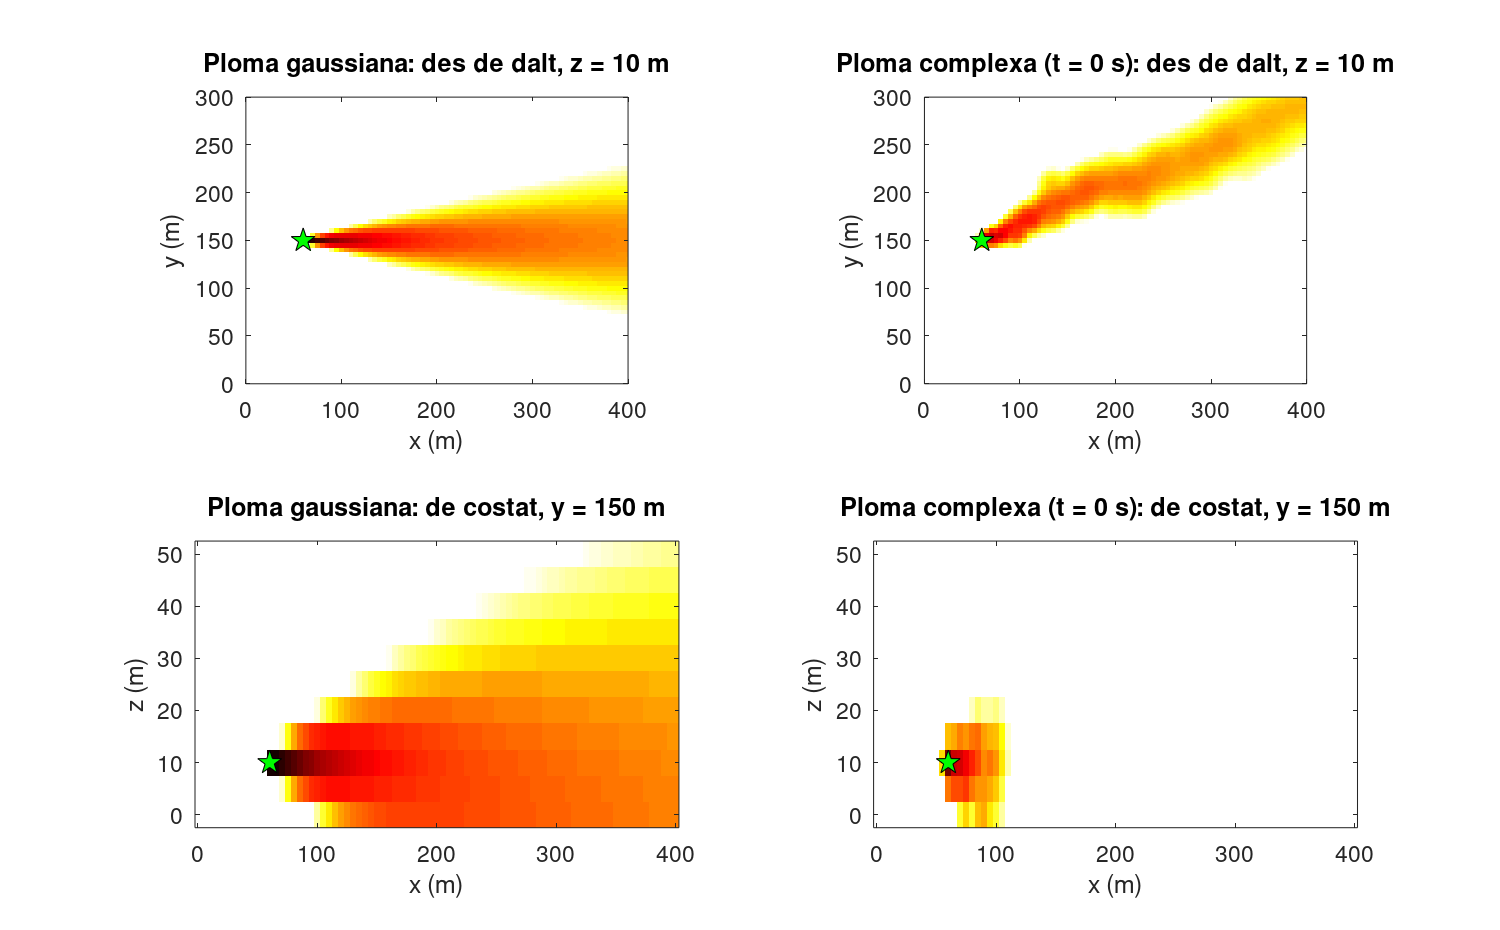
\includegraphics[width=0.95\textwidth]{figures/plomes.png}
\caption{Concentració en escala logarítmica ($\log_{10}$) per a les dues plomes en 3D. A dalt, tall horitzontal a $z = 10$~m; a baix, tall vertical a $y = 150$~m. L'estrella verda és la fuga. La gaussiana és un con simètric i estacionari; la complexa és més estreta, serpenteja i en aquest instant el meandre l'ha desviada cap a $+y$.}
\label{fig:plomes}
\end{figure}

\begin{figure}[htbp]
\centering
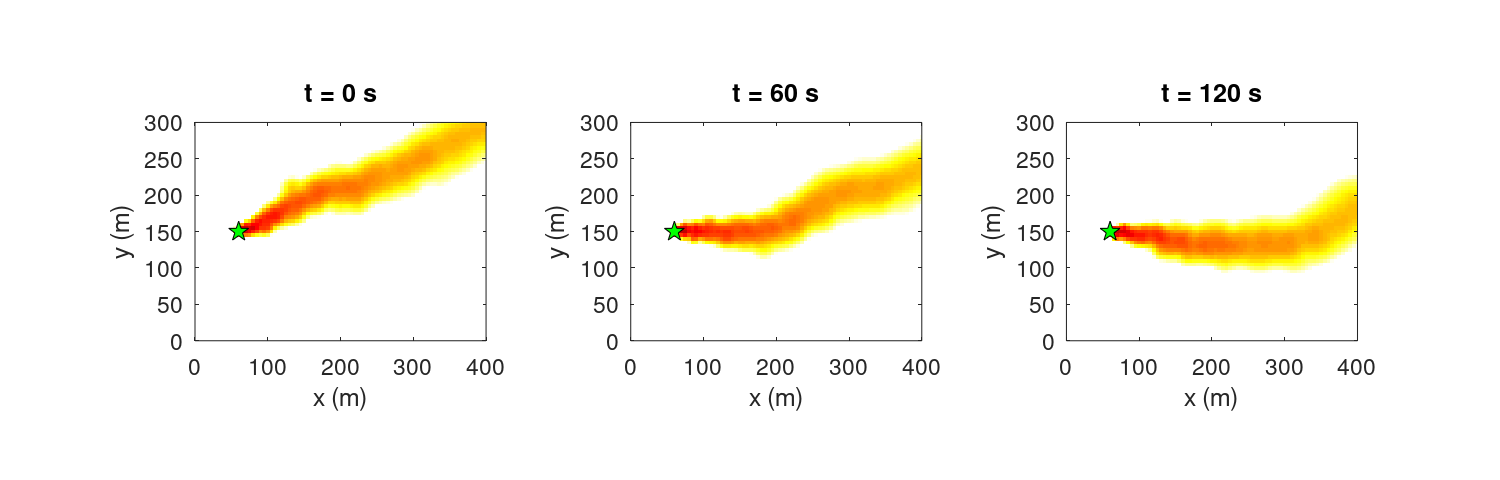
\includegraphics[width=\textwidth]{figures/complexa_temps.png}
\caption{Ploma complexa ($z = 10$~m) en tres instants. El meandre del vent canvia la direcció de la ploma: un punt fix pot passar de ser dins la ploma a ser-ne fora en qüestió de segons.}
\label{fig:temps}
\end{figure}

\section{El dron (\texttt{Dron.m})}

\subsection{Estat i constructor}

El dron es mou per una graella de cel·les de 5~m. A cada pas pot anar a una de les sis cel·les veïnes (est, nord, oest, sud, amunt o avall) o quedar-se quiet; aquests set moviments es guarden a la matriu \texttt{moviments} en format \texttt{[diy dix diz]}. Com que vola a 5~m/s, cada pas dura $\Delta t = 1$~s, i l'autonomia de 2500~s equival a 2500 passos. En 3D vola entre 5 i 40~m d'alçada. El constructor calcula la graella, la cel·la de sortida i el nombre de cel·les visibles a cada costat (\texttt{radiVisible}), i després inicialitza l'estat específic de l'algorisme: el model i el mapa de probabilitat per a l'infotaxis, o els sensors en creu per al gradient (codi~\ref{lst:constructor}). Considerem que el dron troba la fuga quan hi és a menys de 5~m en $x$ i en $y$ i a menys de 2~m en $z$ (mètode \texttt{veuFuga}).

\needspace{15\baselineskip}
\begin{lstlisting}[caption={Inicialització específica de cada algorisme (part del constructor \texttt{Dron}).}, label=lst:constructor]
if strcmp(algorisme, 'infotaxis')
    obj.desplSensors = [0 0 0];      % un sol sensor, al centre del dron
    obj.model = obj.crearModel();
    mapaInicial = ones(g.mida);      % la fuga pot ser a qualsevol lloc...
    mapaInicial(obj.zonaVisible(obj.cel)) = 0;   % ... menys on ja veu
    obj.mapa = mapaInicial / sum(mapaInicial(:));
else
    % Sensors en creu: est, oest, nord, sud i, en 3D, a sobre i a sota
    despl = par.separacioSensors * [1 0 0; -1 0 0; 0 1 0; 0 -1 0; 0 0 1; 0 0 -1];
    obj.desplSensors = despl(1:4 + 2 * strcmp(dimensio, '3d'), :);
    obj.mapa = zeros(g.mida);
    obj.centreZigZag = obj.cel;
    obj.destiTram = obj.cel;
end
\end{lstlisting}

\subsection{Model del sensor}

El sensor és un comptador de deteccions, com un comptador Geiger: a cada pas no dona una concentració sinó un nombre enter de \emph{comptes}, que modelitzem amb una distribució de Poisson. És la distribució del nombre d'esdeveniments independents que passen en un interval amb un ritme mitjà $\lambda$:
\begin{equation}
k \sim \text{Poisson}(\lambda), \qquad \lambda = \Delta t\,(s\,c + b), \qquad P(k \mid \lambda) = \frac{\lambda^k e^{-\lambda}}{k!},
\end{equation}
on $c$ és la concentració, $s = 1$ la sensibilitat i $b = 0{,}02$~comptes/s el fons (falses deteccions). En gran part de la ploma $\lambda \ll 1$ i el resultat més probable és $k = 0$: aquesta és la intermitència que fa difícil el problema. Generem les mostres amb l'algorisme de Knuth, que multiplica números uniformes fins que el producte baixa de $e^{-\lambda}$. Per a $\lambda \geq 30$ fem servir l'aproximació normal $\mathcal{N}(\lambda, \lambda)$, que és més ràpida (codi~\ref{lst:poisson}). Així no depenem de cap \emph{toolbox}.

\needspace{14\baselineskip}
\begin{lstlisting}[caption={Generació de comptes de Poisson (\texttt{Dron.poissonAleatori}).}, label=lst:poisson]
comptes = zeros(size(mitjana));
for i = 1:numel(mitjana)
    if mitjana(i) < 30
        % Metode de Knuth: multiplica numeros a l'atzar fins a baixar de exp(-mitjana)
        producte = rand;
        while producte > exp(-mitjana(i))
            comptes(i) = comptes(i) + 1;
            producte = producte * rand;
        end
    else
        comptes(i) = max(0, round(mitjana(i) + sqrt(mitjana(i)) * randn));   % aproximacio normal
    end
end
\end{lstlisting}

\subsection{Lectura del camp}

Els sensors llegeixen el camp amb interpolació pel \emph{veí més proper}: el punt de la graella i l'instant més propers. Si la simulació dura més que el fitxer, es fa servir l'últim instant, de manera que el mateix codi funciona amb fitxers d'un sol instant; fora del domini del fitxer la concentració és zero (codi~\ref{lst:llegircamp}). L'infotaxis fa servir un sol sensor al centre del dron, i el gradient en fa servir quatre (2D) o sis (3D), en creu, a 5~m del centre.

\needspace{11\baselineskip}
\begin{lstlisting}[caption={Lectura del camp pels sensors (part de \texttt{Dron.llegirCamp}).}, label=lst:llegircamp]
it = Dron.mesProper(camp.t, t);
c  = zeros(size(pos, 1), 1);
for i = 1:size(pos, 1)
    x = pos(i, 1);  y = pos(i, 2);  z = pos(i, 3);
    if x >= camp.x(1) && x <= camp.x(end) && y >= camp.y(1) && y <= camp.y(end)
        c(i) = camp.c(Dron.mesProper(camp.x, x), Dron.mesProper(camp.y, y), ...
                      Dron.mesProper(camp.z, z), it);
    end
end
\end{lstlisting}

\subsection{El mètode \texttt{pas}}

El mètode \texttt{pas} defineix el cicle de cada iteració: \emph{mesurar}, \emph{decidir} i \emph{moure's} (codi~\ref{lst:pas}). La part comuna (sensor i moviment) és igual per als dos algorismes, i la decisió es delega a un mètode privat diferent segons el valor de \texttt{algorisme}. A partir dels comptes, el dron també fa una estimació de la concentració, $\hat c = \max(k/\Delta t - b, 0)/s$, que només es fa servir per a la visualització i per al mapa del gradient.

\needspace{24\baselineskip}
\begin{lstlisting}[caption={Un pas del dron (\texttt{Dron.pas}).}, label=lst:pas]
function pas(obj, camp)
%PAS  Un pas del dron: mesura, decideix on va i s'hi mou.
    p = obj.par;

    % 1. Mesura: comptes de cada sensor
    conc    = Dron.llegirCamp(camp, obj.pos + obj.desplSensors, obj.temps);
    comptes = Dron.poissonAleatori(obj.dt * (p.sensibilitat * conc + p.fonsSensor));
    % concentracio que el dron dedueix dels comptes (mitjana dels sensors)
    obj.concMesurada = mean(max(comptes / obj.dt - p.fonsSensor, 0) / p.sensibilitat);

    % 2. Decideix on va
    if strcmp(obj.algorisme, 'infotaxis')
        obj.infotaxisActualitzar(comptes);
        moviment = obj.infotaxisDecidir();
    else
        c = obj.cel;
        obj.mapa(c(1), c(2), c(3)) = max(obj.mapa(c(1), c(2), c(3)), obj.concMesurada);
        moviment = obj.gradientDecidir(comptes);
    end

    % 3. Es mou a una cel.la veina (o es queda quiet)
    obj.cel = obj.cel + moviment;
    obj.pos = obj.posicio(obj.cel);
    obj.temps = obj.temps + obj.dt;
end
\end{lstlisting}

\section{L'algorisme infotaxis}

L'infotaxis (Vergassola, Villermaux i Shraiman, \emph{Nature} 445, 2007) parteix d'una idea: en una ploma turbulenta el senyal és massa intermitent per seguir-lo, però cada mesura, fins i tot un zero, aporta informació sobre on pot ser la fuga. El dron manté una distribució de probabilitat sobre la posició de la fuga i tria els moviments que maximitzen la informació esperada.

\subsection{Formulació bayesiana}

El dron guarda una probabilitat \emph{a posteriori} $P(\mathbf{r})$ per a cada cel·la $\mathbf{r}$ de la graella, és a dir, la probabilitat que la fuga sigui a $\mathbf{r}$ donades totes les mesures fetes fins ara. La distribució inicial (\emph{a priori}) és uniforme, excepte a les cel·les que el dron ja veu des de la sortida, que tenen probabilitat zero.

\subsection{El model intern del dron}
\label{sec:model}

Per interpretar una mesura, el dron necessita la \emph{versemblança} (\emph{likelihood}): la probabilitat de mesurar $k$ comptes si la fuga fos a $\mathbf{r}$. Això requereix un model de la concentració mitjana. Si la ploma és gaussiana, el model és la mateixa fórmula de Pasquill-Gifford. Si és complexa, fem servir la solució estacionària de l'equació d'advecció-difusió amb decaïment, amb difusivitats efectives anisòtropes i una font imatge:
\begin{equation}
c = \frac{Q}{4\pi\sqrt{D_h D_v}}\, e^{\frac{\Delta x\, U}{2D_h}} \left[\frac{e^{-r_1/\ell}}{r_1} + \frac{e^{-r_2/\ell}}{r_2}\right], \qquad \ell = \sqrt{\frac{D_h\, T}{1 + U^2 T/(4 D_h)}},
\end{equation}
on $r_1$ i $r_2$ són les distàncies a la fuga i a la seva imatge, amb la coordenada vertical escalada per $\sqrt{D_h/D_v}$, $T$ és el temps de vida i $\ell$ la longitud característica. La difusivitat horitzontal efectiva suma la turbulència, el creixement dels puffs i el meandre del vent, $D_h = K_H + G_H + (U\sigma_\theta)^2\tau \approx 11{,}8$~m$^2$/s; el meandre és clarament el terme dominant. La vertical és $D_v = K_V + G_V = 0{,}4$~m$^2$/s. Aquest model descriu la ploma \emph{mitjana}, no la instantània, i és una aproximació deliberada: el dron no coneix la turbulència real.

\textbf{Taula precalculada.} El nombre de comptes esperat només depèn del desplaçament horitzontal entre el dron i la fuga i de les dues alçades (invariància per translació). Per això el calculem una sola vegada al constructor, en una taula de mida $(2n_y-1) \times (2n_x-1) \times n_z \times n_z$; en 3D són $121 \times 161 \times 8 \times 8 \approx 1{,}2$ milions de valors (codi~\ref{lst:model}). Per obtenir els comptes esperats des d'una cel·la per a totes les posicions possibles de la fuga, n'hi ha prou amb extreure un bloc de la taula amb els índexs invertits. Això és equivalent a una correlació, però sense cap càlcul.

\needspace{16\baselineskip}
\begin{lstlisting}[caption={Construcció de la taula del model (\texttt{crearModel}) i extracció dels comptes esperats (\texttt{comptesEsperats}).}, label=lst:model]
        g  = obj.graella;
        ny = g.mida(1);  nx = g.mida(2);  nz = g.mida(3);
        [dx, dy] = meshgrid((-(nx - 1):(nx - 1)) * obj.par.midaCella, ...
                            (-(ny - 1):(ny - 1)) * obj.par.midaCella);
        model = zeros(2 * ny - 1, 2 * nx - 1, nz, nz);
        for izDron = 1:nz
            for izFuga = 1:nz
                conc = obj.concentracioModel(dx, dy, g.z(izDron), g.z(izFuga));
                model(:, :, izDron, izFuga) = obj.dt * (obj.par.sensibilitat * conc + obj.par.fonsSensor);
            end
        end
...
        ny = obj.graella.mida(1);  nx = obj.graella.mida(2);
        esperats = reshape(obj.model(cel(1) + ny - 1:-1:cel(1), cel(2) + nx - 1:-1:cel(2), cel(3), :), ...
                           obj.graella.mida);
\end{lstlisting}

\subsection{Actualització amb la regla de Bayes}

Després de cada mesura, la regla de Bayes actualitza el mapa:
\begin{equation}
P_{\text{nou}}(\mathbf{r}) = \frac{P(\mathbf{r})\, P(k \mid \lambda(\mathbf{r}))}{\sum_{\mathbf{r}'} P(\mathbf{r}')\, P(k \mid \lambda(\mathbf{r}'))},
\end{equation}
on $\lambda(\mathbf{r})$ són els comptes que el model espera si la fuga és a $\mathbf{r}$. A més, les cel·les visibles es posen a zero, perquè si la fuga hi fos el dron ja l'hauria trobada. La versemblança de Poisson es calcula en forma logarítmica, $\exp(-\lambda + k\ln\lambda - \ln k!)$, amb \texttt{gammaln(k+1)} $= \ln k!$, per evitar desbordaments numèrics (codi~\ref{lst:bayes}). Si la mesura és incompatible amb el model a tot arreu (la suma dona zero), només es descarta la zona visible.

\needspace{11\baselineskip}
\begin{lstlisting}[caption={Actualització bayesiana (part de \texttt{Dron.infotaxisActualitzar}).}, label=lst:bayes]
visible  = obj.zonaVisible(obj.cel);
esperats = obj.comptesEsperats(obj.cel);
nou = obj.mapa .* exp(-esperats + comptes * log(esperats) - gammaln(comptes + 1));
nou(visible) = 0;
if sum(nou(:)) == 0                  % mesura que el model no explica:
    nou = obj.mapa;                  % nomes descartem la zona visible
    nou(visible) = 0;
end
obj.mapa = nou / sum(nou(:));
\end{lstlisting}

\subsection{La decisió: minimitzar l'entropia esperada}

La incertesa del mapa es quantifica amb l'\emph{entropia de Shannon}, $S = -\sum_{\mathbf{r}} P(\mathbf{r}) \ln P(\mathbf{r})$, que és màxima quan la probabilitat és uniforme i zero quan la posició de la fuga és certa. Per a cada moviment possible cap a $\mathbf{r}_j$, el dron calcula la variació d'entropia esperada:
\begin{equation}
\overline{\Delta S}(\mathbf{r}_j) = P(\mathbf{r}_j)\,(-S) + \big[1 - P(\mathbf{r}_j)\big] \sum_k \rho_k(\mathbf{r}_j)\, \Delta S_k.
\end{equation}
El primer terme correspon a trobar la fuga en arribar-hi (l'entropia passa a zero). El segon correspon al cas contrari: el dron mesurarà $k$ comptes amb probabilitat predictiva $\rho_k(\mathbf{r}_j) = \sum_{\mathbf{r}} P(\mathbf{r}) P(k \mid \lambda(\mathbf{r}_j \mid \mathbf{r}))$, i l'entropia del mapa actualitzat canviarà $\Delta S_k$. El dron tria el moviment amb el $\overline{\Delta S}$ més negatiu. Aquesta expressió resol de manera natural el dilema entre \emph{explotar} (anar on és més probable que hi hagi la fuga) i \emph{explorar} (anar on la mesura serà més informativa).

Per fer-ho eficient hem aplicat tres optimitzacions (codi~\ref{lst:decidir}):
\begin{itemize}
\item Els comptes s'agrupen en intervals (0, 1, 2, 3--4, 5--7, 8--12\ldots, $\geq 89$), i les probabilitats de Poisson es calculen amb la recurrència $P(k+1) = P(k)\,\lambda/(k+1)$, sense factorials. L'últim interval rep la probabilitat restant.
\item Només es tenen en compte les cel·les amb probabilitat superior a $10^{-15}$, perquè les altres no contribueixen a l'entropia.
\item Quan cap moviment redueix l'entropia ($\overline{\Delta S} > -10^{-6}$), el dron va directament cap a la cel·la més probable. Els empats es trenquen amb una pertorbació aleatòria molt petita.
\end{itemize}

\needspace{33\baselineskip}
\begin{lstlisting}[caption={Probabilitats per intervals i decisió final (part de \texttt{Dron.infotaxisDecidir}).}, label=lst:decidir]
            % Recorrem k = 0, 1, 2... sumant la llei de Poisson interval a interval
            intervals     = obj.par.intervalsComptes;
            canviMesura   = 0;
            probAcumulada = zeros(size(esperats));   % P(comptes < inici de l'interval)
            probK         = exp(-esperats);          % P(k comptes) per al k actual
            k = 0;
            for i = 1:numel(intervals)
                if i < numel(intervals)
                    probInterval = zeros(size(esperats));
                    while k < intervals(i + 1)
                        probInterval = probInterval + probK;
                        probK = probK .* esperats / (k + 1);
                        k = k + 1;
                    end
                    probAcumulada = probAcumulada + probInterval;
                else
                    probInterval = max(1 - probAcumulada, 0);   % ultim interval: la resta
                end
                conjunta   = probSiNo .* probInterval;
                probMesura = sum(conjunta(:));       % probabilitat de mesurar aquest interval
                if probMesura > 1e-300
                    canviMesura = canviMesura + probMesura * (Dron.entropia(conjunta / probMesura) - S);
                end
            end
            canvi(m) = probTrobar * (-S) + (1 - probTrobar) * canviMesura;
...
        if min(canvi) > -1e-6
            % Ja no pot aprendre res mes: va directe al punt mes probable
            obj.queFa = 'cap al punt mes probable';
            [~, idx] = max(prob(:));
            [iy, ix, iz] = ind2sub(g.mida, idx);
            moviment = Dron.pasCapA(obj.cel, [iy ix iz]);
        else
            obj.queFa = 'infotaxis';
            [~, millor] = min(canvi + 1e-10 * abs(S) * rand(7, 1));   % desempat a l'atzar
            moviment = g.moviments(millor, :);
        end
\end{lstlisting}

La figura~\ref{fig:inf2d} mostra l'evolució del mapa en el cas 2D amb ploma gaussiana. Als 20~s el dron gairebé no ha detectat res, però la falta de deteccions ja és informativa: la zona blanca correspon a posicions on la ploma hauria passat pel lloc on ha volat el dron, i per tant són poc probables. Als 60~s la probabilitat ja es concentra en una franja vent amunt al voltant de $y = 150$~m. La figura~\ref{fig:inf3d120} mostra el cas 3D: el mapa des de dalt suma la probabilitat de totes les alçades, i la trajectòria mostra com el dron explora també en vertical.

\begin{figure}[htbp]
\centering
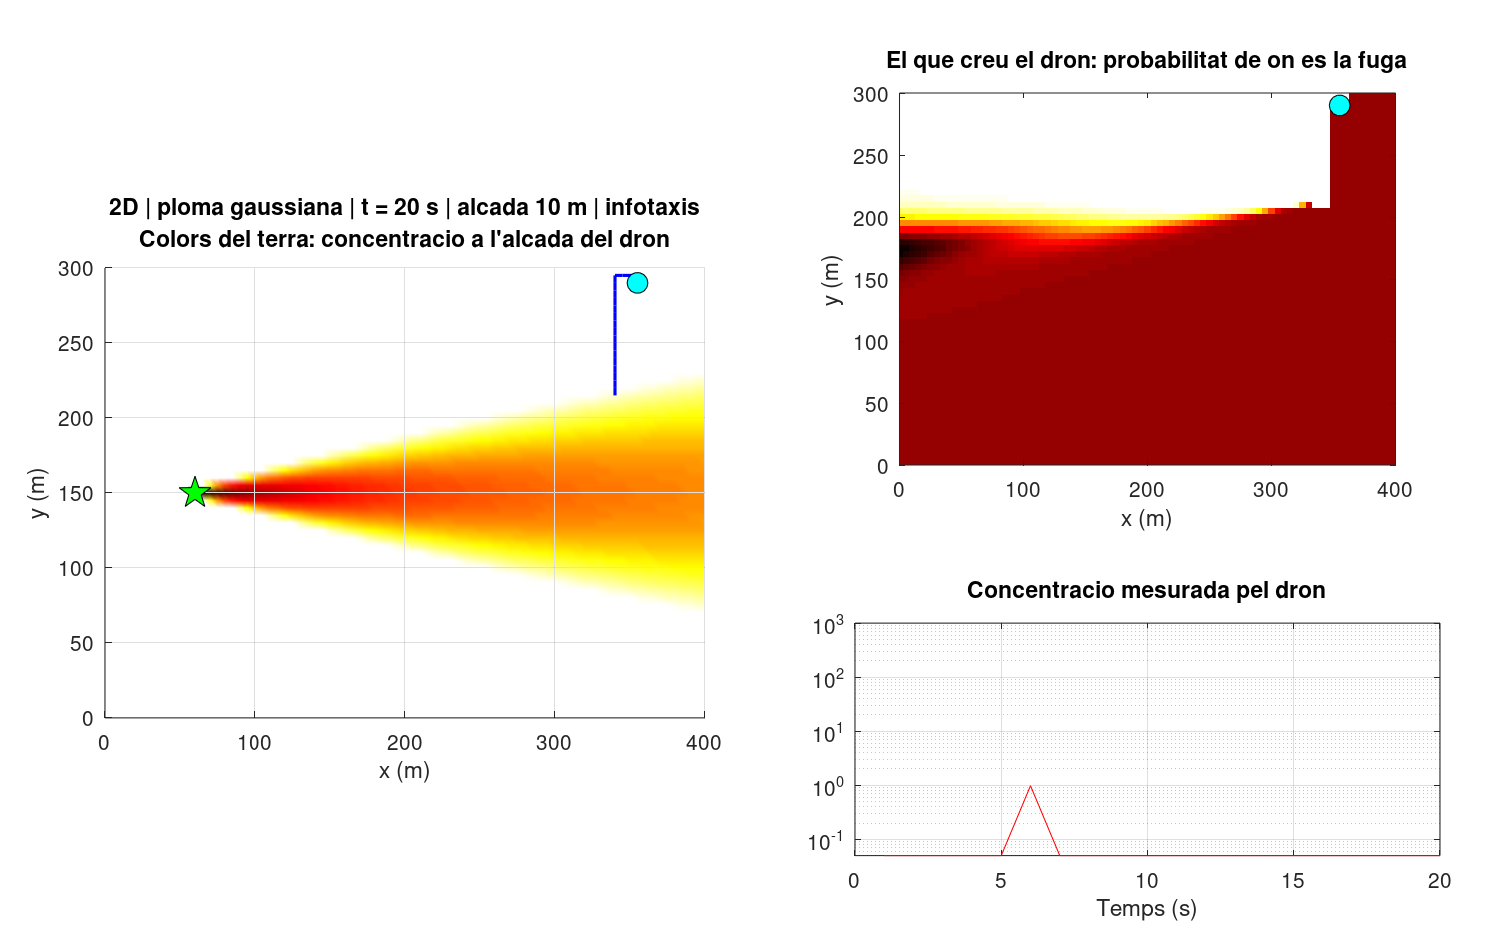
\includegraphics[width=0.76\textwidth]{figures/g2d_inf_t020.png}\\[4pt]
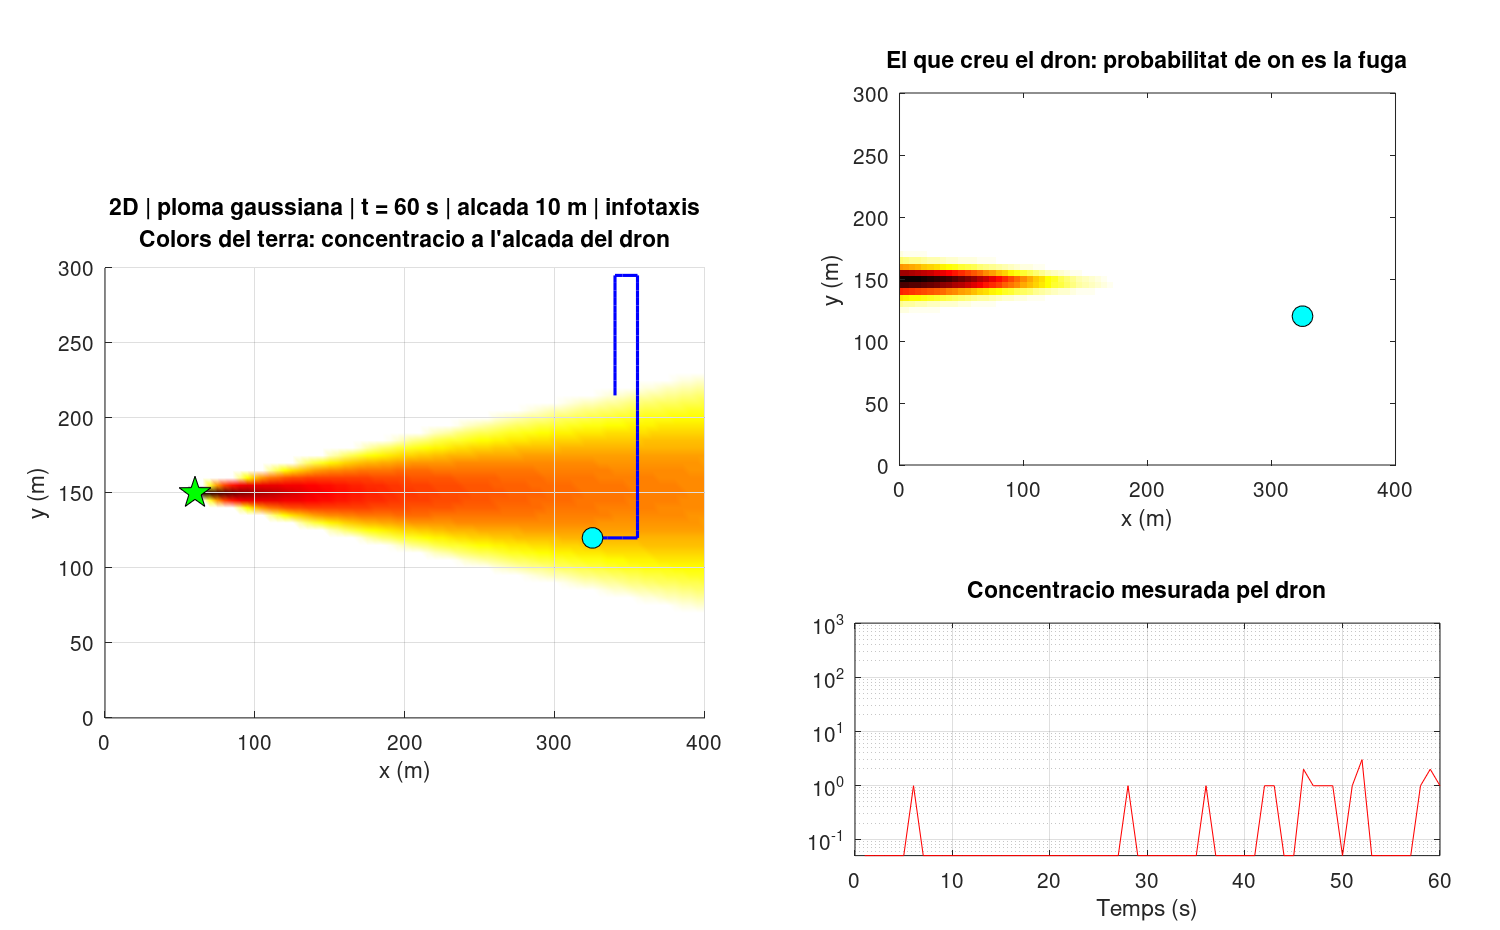
\includegraphics[width=0.76\textwidth]{figures/g2d_inf_t060.png}
\caption{Infotaxis en 2D amb ploma gaussiana, als 20~s (a dalt) i als 60~s (a baix). Panells: escena real amb la ploma, la fuga (estrella), el dron (cercle) i la trajectòria; mapa de probabilitat del dron (més fosc, més probable); concentració estimada pel dron al llarg del temps.}
\label{fig:inf2d}
\end{figure}

\begin{figure}[htbp]
\centering
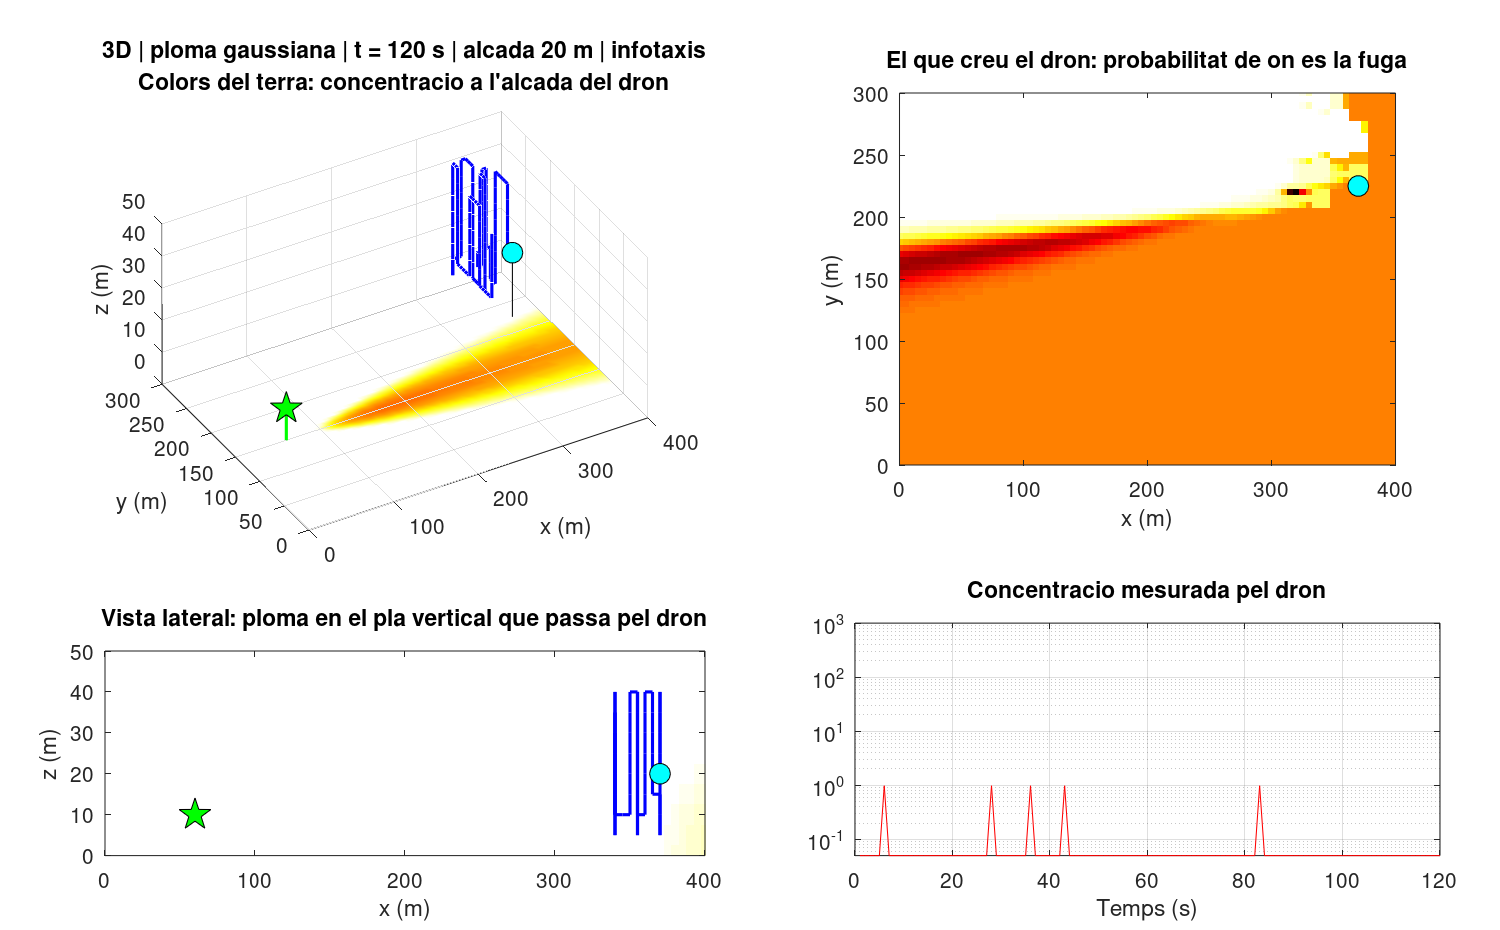
\includegraphics[width=0.76\textwidth]{figures/g3d_inf_t120.png}
\caption{Infotaxis en 3D amb ploma gaussiana als 120~s. El dron ha explorat diverses alçades a prop del punt de sortida (vista lateral, a baix a l'esquerra) i el mapa ja concentra la probabilitat vent amunt, entre $y \approx 150$ i 180~m.}
\label{fig:inf3d120}
\end{figure}

\section{L'algorisme del gradient}

\subsection{Estimació del gradient}

L'algorisme del gradient és una estratègia reactiva, inspirada en la quimiotaxi (el moviment d'organismes guiat per un gradient químic). El dron porta sensors en creu a una distància $d = 5$~m del centre i estima el gradient amb diferències finites centrades:
\begin{equation}
\frac{\partial c}{\partial x} \approx \frac{c_{\text{est}} - c_{\text{oest}}}{2d}, \qquad \frac{\partial c}{\partial y} \approx \frac{c_{\text{nord}} - c_{\text{sud}}}{2d}, \qquad \frac{\partial c}{\partial z} \approx \frac{c_{\text{sobre}} - c_{\text{sota}}}{2d}.
\end{equation}
Com que les estimacions són molt sorolloses, les suavitzem amb una mitjana mòbil exponencial (\emph{EMA}), un filtre passa-baix de primer ordre, $\mathbf{g}_n = \alpha\,\mathbf{g}_{n-1} + (1-\alpha)\,\mathbf{g}_{\text{nou}}$, amb $\alpha = 0{,}6$ (codi~\ref{lst:gradest}). El vector de concentracions dels sensors està ordenat en parells oposats (est, oest, nord, sud, sobre, sota), de manera que \texttt{conc(1:2:end) - conc(2:2:end)} calcula totes les diferències de cop.

\needspace{16\baselineskip}
\begin{lstlisting}[caption={Estimació i filtratge del gradient, i detecció del senyal (part de \texttt{Dron.gradientDecidir}).}, label=lst:gradest]
conc = max(comptes(:)' / obj.dt - p.fonsSensor, 0) / p.sensibilitat;   % concentracio a cada sensor
gradientNou = [0 0 0];
gradientNou(1:numel(conc) / 2) = (conc(1:2:end) - conc(2:2:end)) / (2 * p.separacioSensors);
passosMemoria = round(p.tempsMemoria / obj.dt);   % passos que recorda el senyal

if sum(comptes) >= p.llindarDeteccio * obj.dt
    obj.passosSenseSenyal = 0;
    obj.gradientFiltrat = p.suavitzat * obj.gradientFiltrat + (1 - p.suavitzat) * gradientNou;
    obj.centreZigZag = obj.cel;      % si perd el senyal, el buscara al voltant d'aqui
    obj.tram = 0;
else
    obj.passosSenseSenyal = obj.passosSenseSenyal + 1;
    if obj.passosSenseSenyal > passosMemoria
        obj.gradientFiltrat = [0 0 0];   % senyal perdut: oblida el gradient
    end
end
\end{lstlisting}

\subsection{Màquina d'estats: seguir o buscar}

El comportament és una \emph{màquina d'estats finits} amb dos estats (figura~\ref{fig:estats}). Considerem que hi ha senyal quan la suma de comptes de tots els sensors arriba a 2~comptes/s.
\begin{itemize}
\item \textbf{Seguint el gradient.} Mentre hi ha hagut senyal en els últims 4~s, el dron projecta el gradient filtrat sobre els sis moviments possibles (producte escalar) i tria el de projecció màxima. El moviment vent avall està prohibit, perquè la fuga sempre és vent amunt.
\item \textbf{Buscant en zig-zag.} Si passen 4~s sense senyal, s'oblida el gradient i comença una cerca de traves al vent al voltant del punt on ha perdut la ploma, com fan les arnes quan segueixen una feromona (\emph{casting}). Els trams alternen de costat i l'amplitud creix geomètricament, $A_n = 20 \cdot 2^{n-1}$~m. En 3D, cada tram també canvia d'alçada, alternativament per sobre i per sota. Quan torna a detectar senyal, el zig-zag es reinicia.
\end{itemize}

\begin{figure}[htbp]
\centering
\begin{tikzpicture}[estat/.style={draw=MidnightBlue, fill=MidnightBlue!8, rounded corners=6pt, minimum width=36mm, minimum height=11mm, align=center, font=\small}, fletxa/.style={-{Stealth[length=2.5mm]}, thick}]
\node[estat] (seg) {Seguint el gradient};
\node[estat, right=40mm of seg] (zz) {Buscant en zig-zag};
\draw[fletxa] (seg.north east) to[bend left=18] node[above, font=\footnotesize]{4~s sense senyal} (zz.north west);
\draw[fletxa] (zz.south west) to[bend left=18] node[below, font=\footnotesize]{detecta senyal} (seg.south east);
\draw[fletxa] (seg.west) to[out=150, in=210, looseness=5] node[left, font=\footnotesize, align=center]{senyal\\recent} (seg.west);
\draw[fletxa] (zz.east) to[out=30, in=-30, looseness=5] node[right, font=\footnotesize, align=center]{tram nou\\$A_n = 20\cdot 2^{n-1}$~m} (zz.east);
\end{tikzpicture}
\caption{Màquina d'estats de l'algorisme del gradient.}
\label{fig:estats}
\end{figure}

\needspace{20\baselineskip}
\begin{lstlisting}[caption={Decisió del gradient en cada estat (part de \texttt{Dron.gradientDecidir}).}, label=lst:gradient]
if obj.passosSenseSenyal <= passosMemoria
    obj.queFa = 'seguint el gradient';
    veines    = obj.cel + g.moviments(1:6, :);
    dinsZona  = all(veines >= 1, 2) & all(veines <= g.mida, 2);
    projeccio = g.moviments(1:6, [2 1 3]) * obj.gradientFiltrat' + 1e-12 * rand(6, 1);   % gradient en cada direccio
    projeccio(~dinsZona) = -Inf;
    projeccio(1) = -Inf;             % mai vent avall
    [~, millor] = max(projeccio);
    moviment = g.moviments(millor, :);
else
    obj.queFa = 'buscant la ploma en zig-zag';
    if obj.tram == 0 || isequal(obj.cel, obj.destiTram)
        % Tram nou: cap a l'altre costat, el doble de lluny i a una altra alcada
        obj.tram = obj.tram + 1;
        amplitud = max(1, round(p.tramInicial / p.midaCella)) * 2^(obj.tram - 1);    % en cel.les
        canviZ   = round(p.canviAlcadaZigZag / p.midaCella) * floor(obj.tram / 2);  % en cel.les
        costat   = (-1)^obj.tram;
        obj.destiTram = min(max(obj.centreZigZag + costat * [amplitud 0 canviZ], 1), g.mida);
    end
    moviment = Dron.pasCapA(obj.cel, obj.destiTram);
\end{lstlisting}

\section{Bucle de simulació i visualització (\texttt{main.m})}

La funció \texttt{simular} crea l'objecte \texttt{Dron} i executa el bucle principal (codi~\ref{lst:bucle}). A cada iteració el dron fa un pas, es comprova la condició d'èxit i es desa la trajectòria. El bucle acaba quan es troba la fuga o s'exhaureix l'autonomia. La funció retorna una \emph{struct} \texttt{res} amb el resultat (\texttt{trobada}, \texttt{temps}, \texttt{recorregut}, \texttt{distanciaFinal} i \texttt{trajectoria}), separada de la visualització. Així es pot executar sense gràfics i encadenar moltes simulacions.

\needspace{19\baselineskip}
\begin{lstlisting}[caption={Bucle principal de \texttt{simular}.}, label=lst:bucle]
for pas = 1:dron.maxPassos
    dron.pas(camp);                              % el dron mesura, decideix i es mou
    trobada = dron.veuFuga(camp.posFuga);        % ha arribat a la fuga?

    trajectoria(pas + 1, :) = dron.pos;
    concMesurada(pas) = dron.concMesurada;

    if opcions.animacio && (trobada || mod(pas, max(1, round(opcions.dibuixaCada / dron.dt))) == 0)
        if ~ishandle(fig.finestra)
            break;                               % s'ha tancat la finestra
        end
        titol = sprintf('%s | ploma %s | t = %.0f s | alcada %.0f m | %s', upper(opcions.dimensio), ...
                        opcions.tipusPloma, dron.temps, dron.pos(3), dron.queFa);
        actualitzar_figura(fig, camp, dron, trajectoria(1:pas + 1, :), concMesurada(1:pas), titol);
    end
    if trobada
        break;
    end
end
\end{lstlisting}

La visualització segueix un patró eficient. \texttt{crear\_figura} crea una sola vegada tots els objectes gràfics (superfícies, línies, marcadors) i en desa els \emph{handles}, que són referències a aquests objectes. Després, \texttt{actualitzar\_figura} només en modifica les dades amb \texttt{set} (codi~\ref{lst:dibuix}). Això és molt més ràpid que tornar a dibuixar la figura sencera a cada pas. La figura té quatre panells: l'escena real (el tall de la ploma a l'alçada del dron pintat al terra, la fuga, el dron i la trajectòria), una vista lateral en 3D, el coneixement del dron (el mapa de probabilitat o la concentració màxima mesurada a cada cel·la) i la sèrie temporal de concentració mesurada.

\needspace{8\baselineskip}
\begin{lstlisting}[caption={Actualització dels objectes gràfics amb \texttt{set} (part d'\texttt{actualitzar\_figura}).}, label=lst:dibuix]
% Escena real: tall horitzontal de la matriu a l'alcada del dron
set(fig.terra, 'CData', log10(double(camp.c(:, :, iz, it))' + 1e-3));
set(fig.trajectoria, 'XData', trajectoria(:, 1), 'YData', trajectoria(:, 2), 'ZData', trajectoria(:, 3));
set(fig.pal,  'XData', p(1) * [1 1], 'YData', p(2) * [1 1], 'ZData', [0 p(3)]);
set(fig.dron, 'XData', p(1), 'YData', p(2), 'ZData', p(3));
\end{lstlisting}

\section{Resultats}

\subsection{Comparació dels vuit casos}

La taula~\ref{tab:resultats} i la figura~\ref{fig:barres} recullen els resultats dels vuit casos amb la llavor 1. Definim l'\emph{índex de recorregut} com la distància recorreguda dividida pel camí mínim (335~m en 2D, 355~m en 3D): un índex de 2 vol dir que el dron ha recorregut el doble del necessari.

\begin{table}[htbp]
\centering
\caption{Resultats dels vuit casos (llavor 1). En tots els casos el dron troba la fuga.}
\label{tab:resultats}
\begin{tabular}{@{}lllrrr@{}}
\toprule
Dimensió & Ploma & Algorisme & Temps (s) & Recorregut (m) & Índex \\
\midrule
2D & gaussiana & infotaxis & 130 & 630 & 1,9 \\
2D & gaussiana & gradient & 196 & 980 & 2,9 \\
2D & complexa & infotaxis & 279 & 1395 & 4,2 \\
2D & complexa & gradient & 228 & 1140 & 3,4 \\
\midrule
3D & gaussiana & infotaxis & 255 & 1250 & 3,5 \\
3D & gaussiana & gradient & 346 & 1730 & 4,9 \\
3D & complexa & infotaxis & 307 & 1535 & 4,3 \\
3D & complexa & gradient & 275 & 1375 & 3,9 \\
\bottomrule
\end{tabular}
\end{table}

\begin{figure}[htbp]
\centering
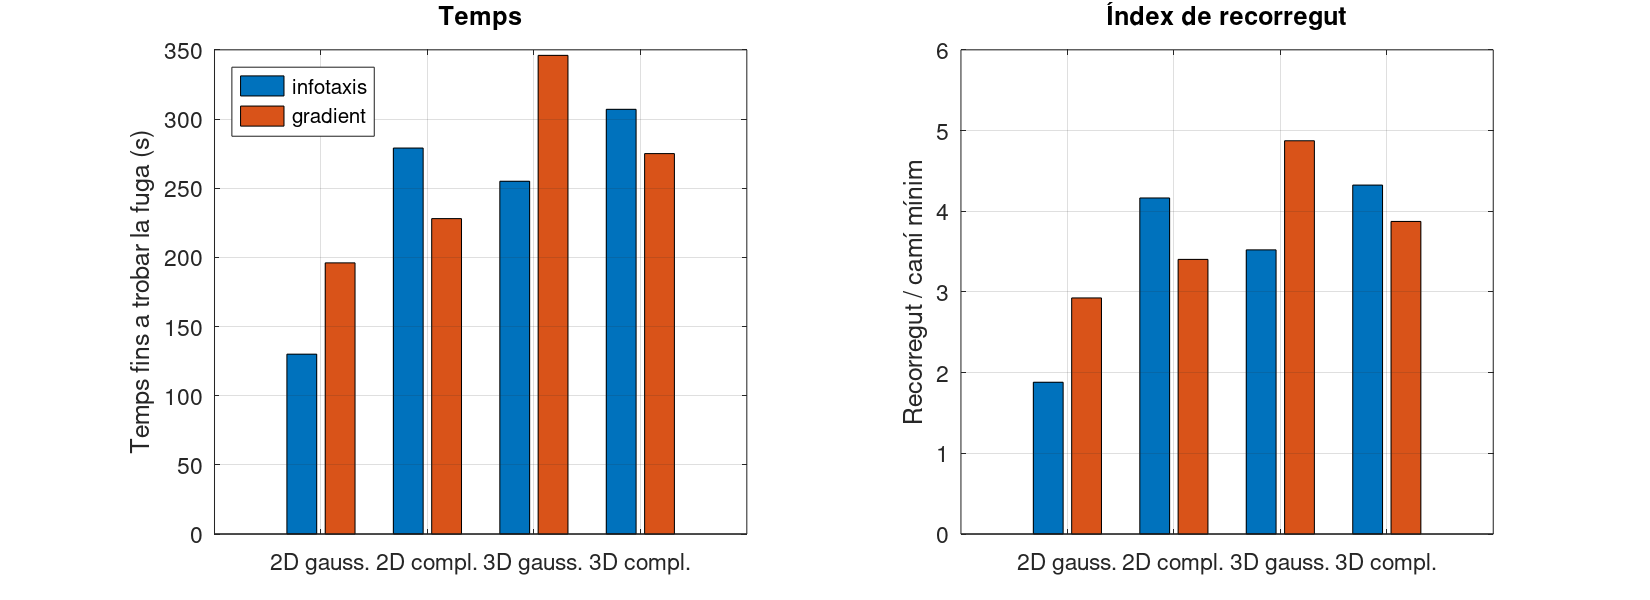
\includegraphics[width=\textwidth]{figures/barres.png}
\caption{Temps fins a trobar la fuga i índex de recorregut per als quatre escenaris i els dos algorismes.}
\label{fig:barres}
\end{figure}

Amb la ploma gaussiana, l'infotaxis és més ràpid que el gradient tant en 2D com en 3D. És l'escenari ideal per a l'infotaxis, perquè el seu model coincideix exactament amb la ploma real i la inferència bayesiana és exacta. Amb la ploma complexa, en canvi, el gradient ha estat més ràpid en aquesta llavor. Els casos 3D són més costosos perquè l'espai de cerca és vuit vegades més gran i el dron també ha d'estimar l'alçada de la fuga.

\subsection{Ploma complexa}

La figura~\ref{fig:c2d} compara els dos algorismes sobre la mateixa ploma complexa en 2D. Als 120~s, l'infotaxis concentra la probabilitat al voltant de $y \approx 200$~m, desplaçada respecte a la fuga real ($y = 150$~m): probablement, les poques deteccions que ha tingut corresponen a moments en què el meandre desviava la ploma cap a $+y$, i el model mitjà les interpreta com si la fuga fos més al nord. El gradient, en canvi, combina trams de zig-zag sense senyal amb trams de remuntada quan entra a la ploma, i la concentració que mesura creix a mesura que s'acosta a la fuga.

\begin{figure}[htbp]
\centering
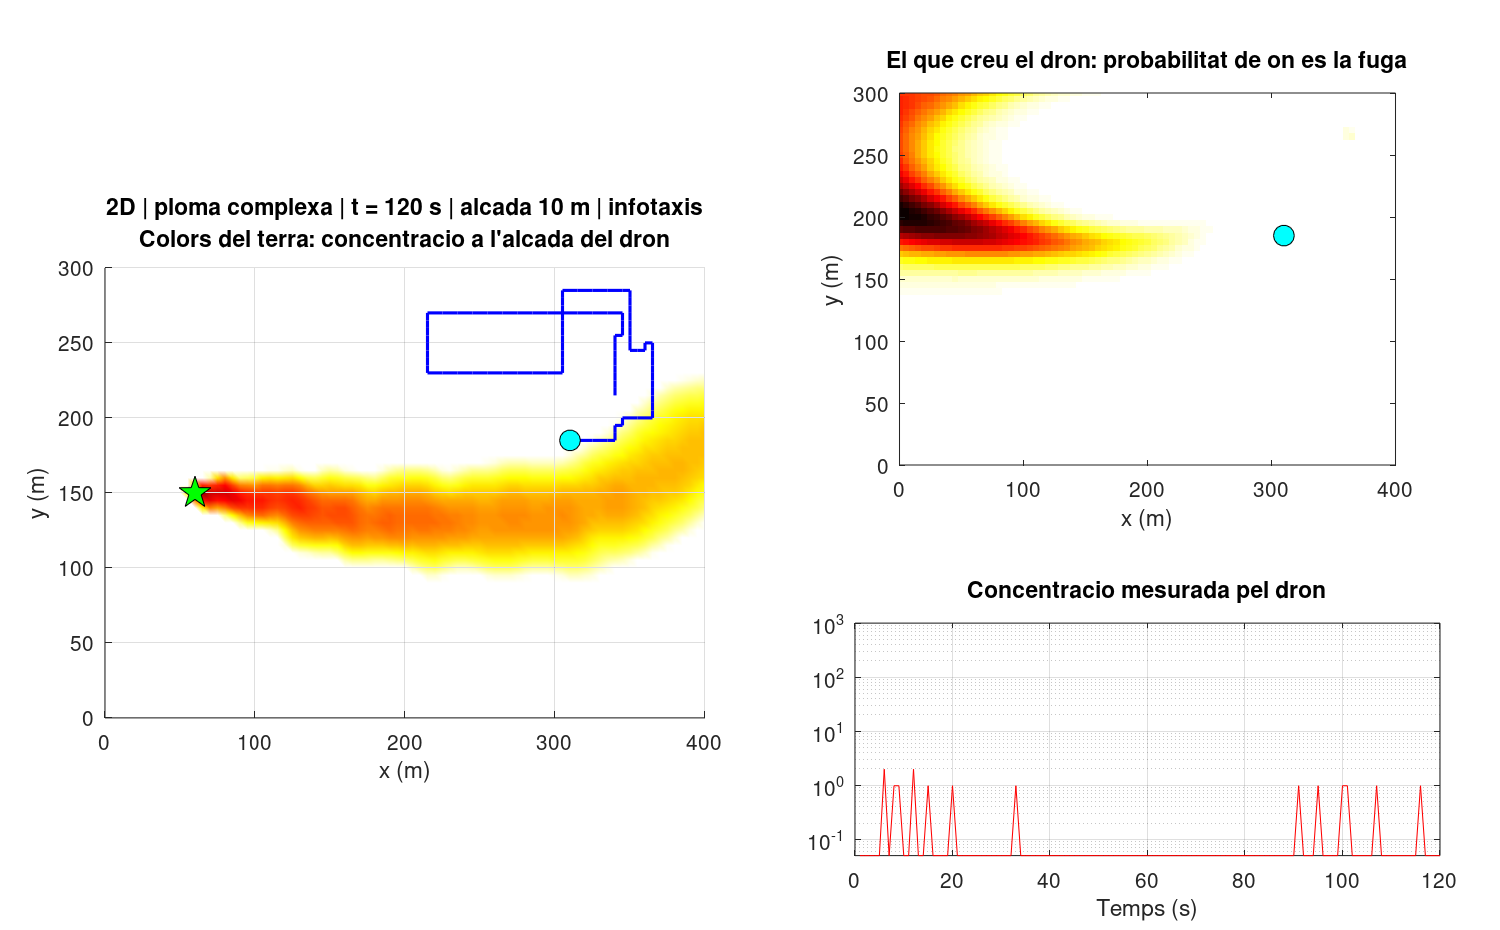
\includegraphics[width=0.76\textwidth]{figures/c2d_inf_t120.png}\\[4pt]
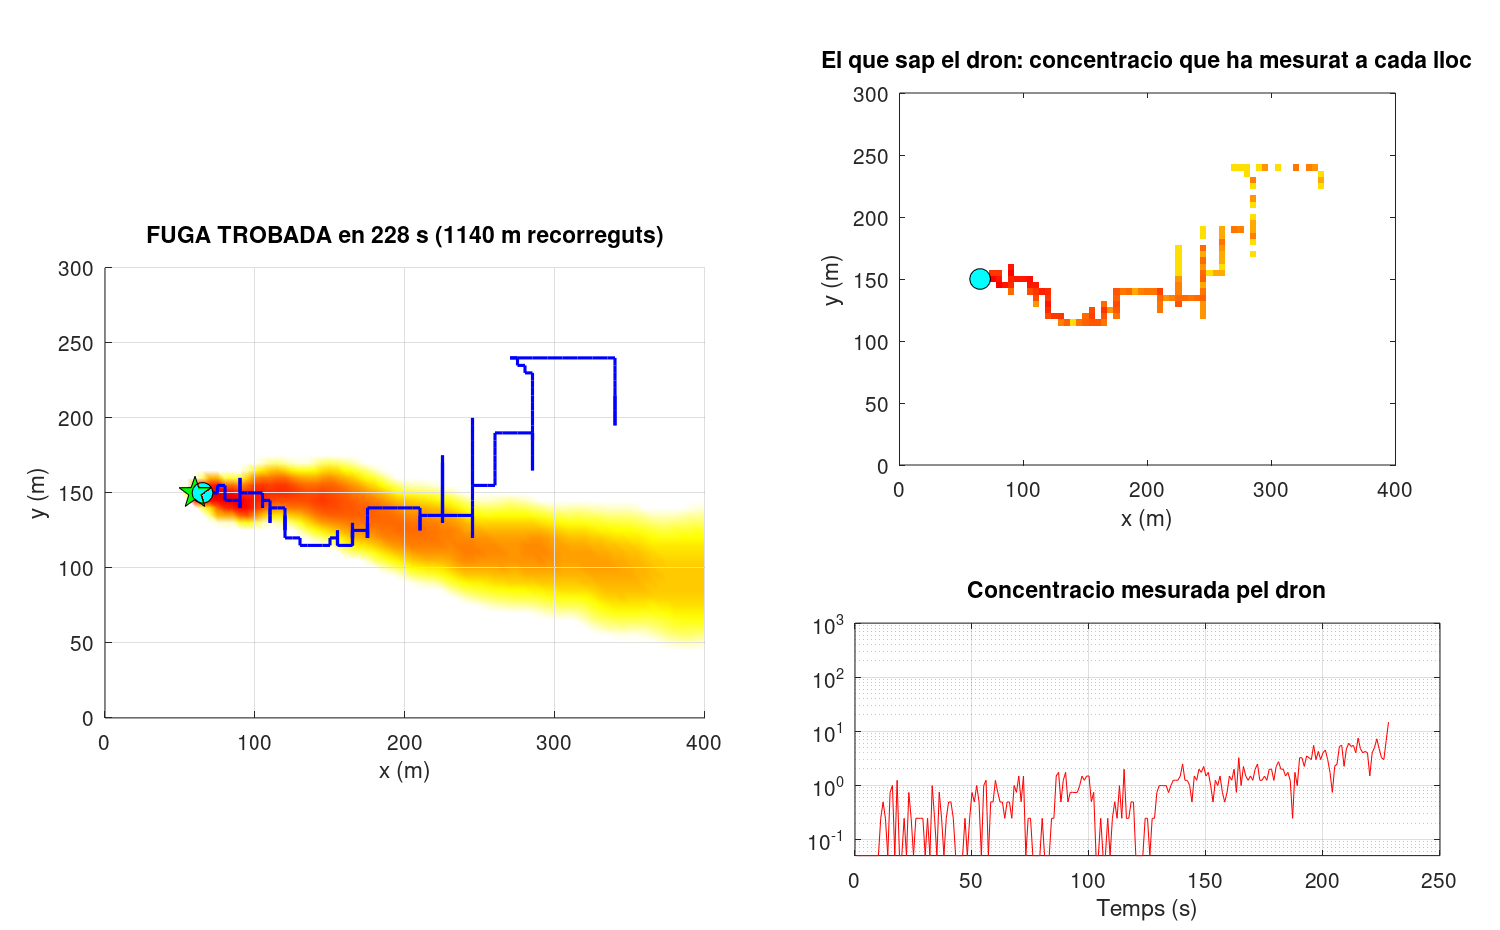
\includegraphics[width=0.76\textwidth]{figures/c2d_grad_final.png}
\caption{Ploma complexa en 2D. A dalt, infotaxis als 120~s; a baix, gradient en el moment de trobar la fuga (228~s). En el gradient, el panell de dalt a la dreta mostra la concentració màxima mesurada a cada cel·la.}
\label{fig:c2d}
\end{figure}

En 3D (figures~\ref{fig:c3dg} i~\ref{fig:c3di}) el patró és similar. El gradient alterna cerca en zig-zag, en horitzontal i en vertical, amb remuntades de la ploma. L'infotaxis, als 200~s, creu que la fuga és a prop de $(155, 120)$~m, quan en realitat és a $(60, 150)$~m. Quan el dron entra en una branca desviada de la ploma i hi mesura molts comptes, el model mitjà, que suposa una ploma recta i centrada, interpreta que la fuga és a prop. En arribar-hi i no trobar-la, la regla de Bayes descarta aquella zona i el dron continua vent amunt fins que la troba als 307~s. Aquest és el límit principal de l'infotaxis: la seva eficiència depèn de la qualitat del model de la ploma.

\begin{figure}[htbp]
\centering
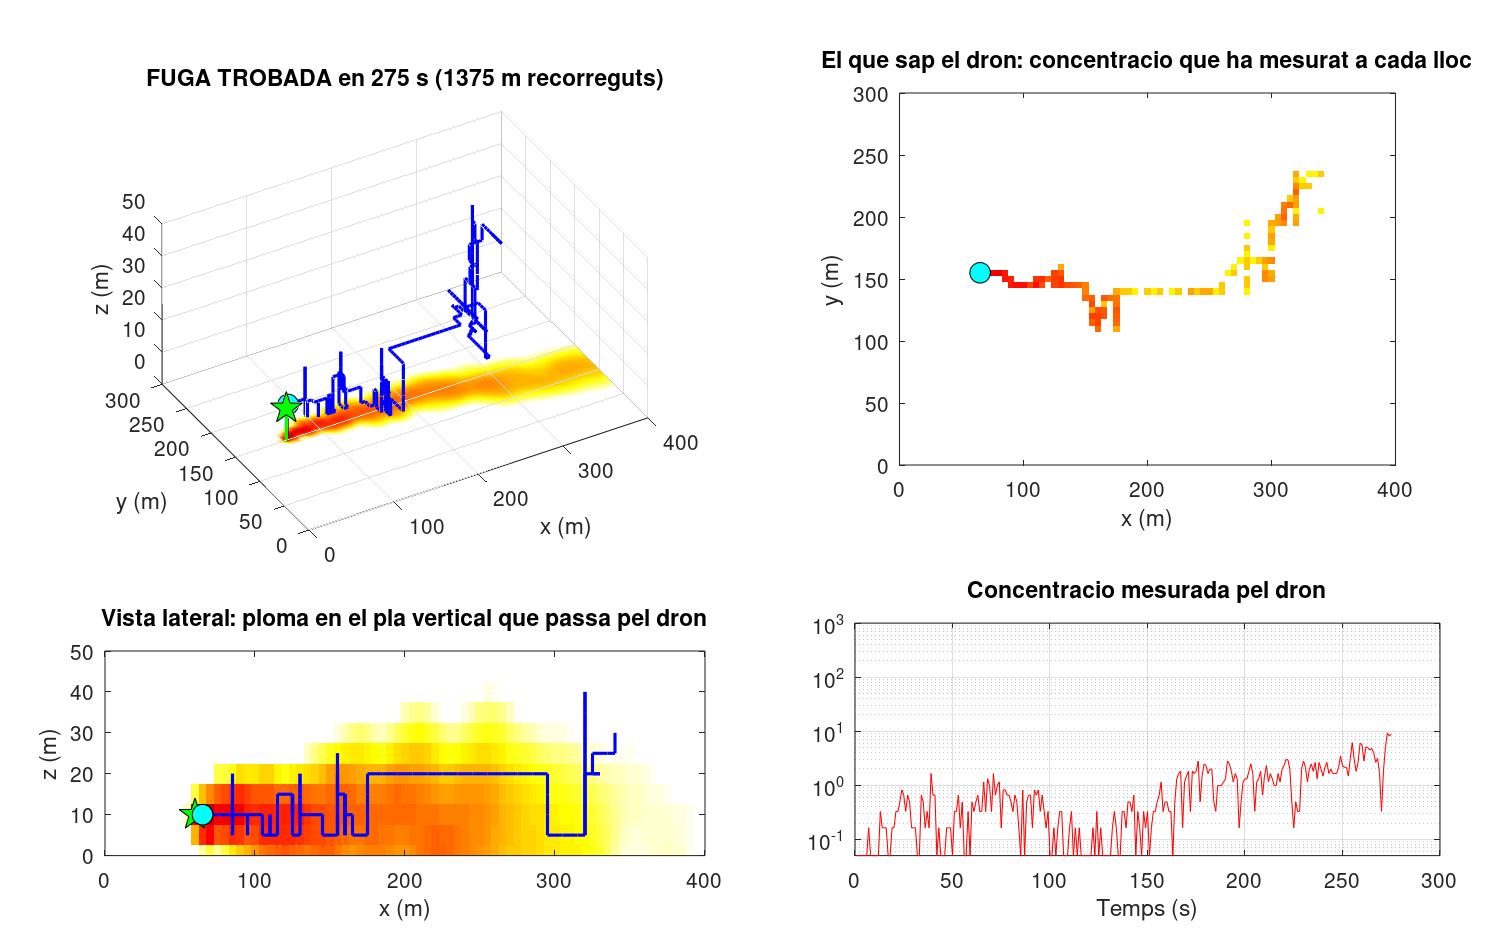
\includegraphics[width=0.76\textwidth]{figures/c3d_grad_final.png}
\caption{Gradient en 3D amb ploma complexa, en el moment de trobar la fuga (275~s).}
\label{fig:c3dg}
\end{figure}

\begin{figure}[htbp]
\centering
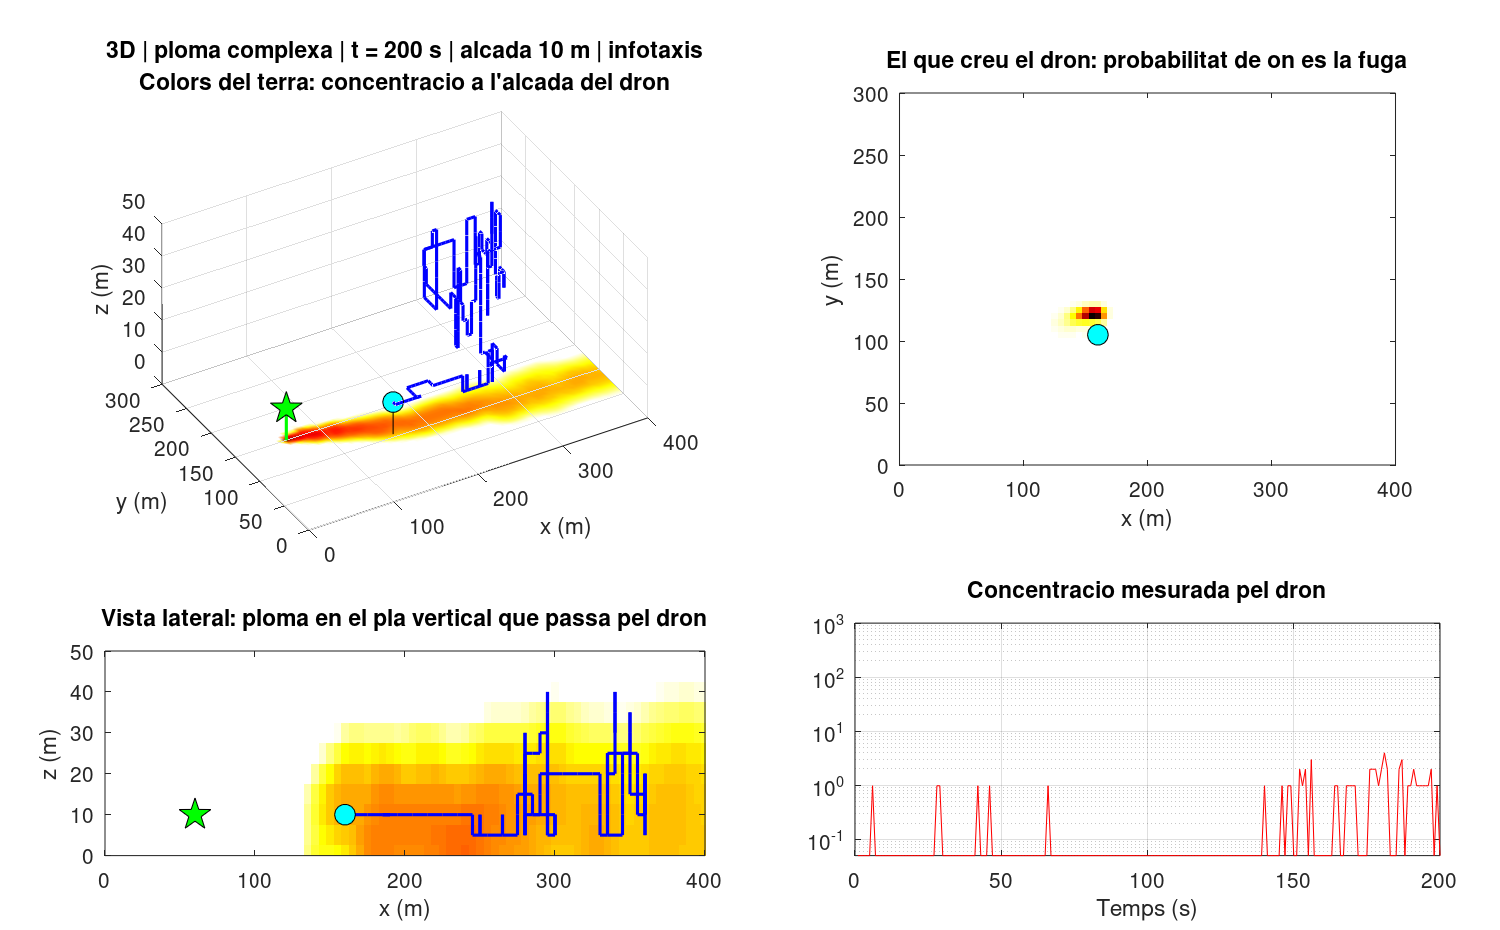
\includegraphics[width=0.76\textwidth]{figures/c3d_inf_t200.png}
\caption{Infotaxis en 3D amb ploma complexa als 200~s. La probabilitat (a dalt a la dreta) es concentra en una posició equivocada, a prop de $(155, 120)$~m; el dron acaba trobant la fuga als 307~s.}
\label{fig:c3di}
\end{figure}

\subsection{Cost computacional}

El cost per pas dels dos algorismes és molt diferent. A cada pas, l'infotaxis avalua set moviments i, per a cadascun, recorre tots els intervals de comptes sobre totes les posicions possibles de la fuga, que en 3D són fins a $61 \times 81 \times 8 \approx 4 \cdot 10^4$ cel·les. Això fa que un pas en 3D costi desenes de mil·lisegons. El gradient només fa unes quantes operacions aritmètiques per pas, de l'ordre d'un mil·lisegon, gairebé tot dedicat a llegir els sensors. La generació de la ploma complexa en 3D i l'escriptura del fitxer NetCDF triguen pocs segons gràcies a la formulació separable.

\section{Treball futur}

\begin{itemize}
\item \textbf{Estudi de Monte Carlo.} Els resultats de la taula~\ref{tab:resultats} corresponen a una sola realització per cas, i amb una altra llavor podrien canviar. El pas següent és repetir cada cas amb moltes plomes, posicions de la fuga i punts de sortida aleatoris, i comparar estadístics com la taxa d'èxit, el temps mitjà i la seva dispersió. Com que \texttt{simular} retorna una \emph{struct} i pot executar-se sense gràfics, n'hi ha prou amb un bucle exterior.
\item \textbf{Plomes realistes.} Disposem d'una simulació de grans remolins (LES, \emph{Large-Eddy Simulation}) feta amb el model PALM de la dispersió de PM10 al parc de tancs del port de Tarragona. És un fitxer NetCDF d'un sol instant, amb una graella de $750 \times 750 \times 202$ punts a 1~m de resolució horitzontal, la concentració \texttt{kc\_PM10} en kg/m$^3$ i les dimensions en el mateix ordre que les nostres. Per integrar-lo caldrà adaptar \texttt{Ploma.llegir} als noms de les variables (per exemple, \texttt{zu\_3d} per a l'alçada), ajustar la sensibilitat del sensor a les unitats físiques i tenir en compte la mida (uns $1{,}1 \cdot 10^8$ valors, 450~MB en precisió simple), possiblement llegint només un subdomini. Com que és un sol instant, el dron veurà una ploma congelada.
\item \textbf{Model de l'infotaxis.} Amb plomes realistes el dron no coneixerà exactament la taxa d'emissió ni les difusivitats. Caldrà estudiar la sensibilitat de l'infotaxis als errors del model, o bé estimar els paràmetres a partir de les mateixes mesures.
\item \textbf{Simplificacions del dron.} El dron es mou només paral·lel als eixos, coneix perfectament la direcció mitjana del vent i els sensors fan servir el veí més proper. Es podrien afegir moviments diagonals, interpolació trilineal i soroll en la mesura del vent.
\end{itemize}

\end{document}
